%
% $RCSfile: pattern.tex,v $
%
% Copyright (C) 2002-2008. Christian Heller.
%
% Permission is granted to copy, distribute and/or modify this document
% under the terms of the GNU Free Documentation License, Version 1.1 or
% any later version published by the Free Software Foundation; with no
% Invariant Sections, with no Front-Cover Texts and with no Back-Cover
% Texts. A copy of the license is included in the section entitled
% "GNU Free Documentation License".
%
% http://www.cybop.net
% - Cybernetics Oriented Programming -
%
% http://www.resmedicinae.org
% - Information in Medicine -
%
% Version: $Revision: 1.1 $ $Date: 2008-08-19 20:41:08 $ $Author: christian $
% Authors: Christian Heller <christian.heller@tuxtax.de>
%

\section{Pattern}
\label{pattern_heading}
\index{Pattern}
\index{Design Technique}
\index{Software Pattern}
\index{Object Oriented Programming}
\index{OOP}
\index{Gang of Four}
\index{GoF}
\index{Anti Pattern}
\index{Amelioration Pattern}
\index{Pattern Language}
\index{Pattern System}
\index{Software Pattern Classification}
\index{Architectural Pattern}
\index{Design Pattern}
\index{Idiomatic Pattern}
\index{Creational Design Pattern}
\index{Structural Design Pattern}
\index{Behavioural Design Pattern}
\index{Fundamental Pattern}
\index{Concurrency Pattern}
\index{Real Time Pattern}
\index{Analysis Pattern}
\index{Meta Model Pattern}

The previous sections investigated basic concepts offered by today's
programming languages and -paradigms. The following and all later sections of
this chapter describe design techniques that belong to a higher conceptual
level. \emph{Patterns}, in a more correct form called \emph{Software Patterns},
are the first technique dealt with. They became popular through
\emph{Object Oriented Programming} (OOP), but their use is not limited to OOP
languages. Patterns represent solutions for recurring software design problems
and can be understood as recommendations for how to build software in an
elegant and efficient way. In the past, more detailed definitions have been
given by meanwhile well-known authors.

Christopher Alexander, an architect and urban planner, writes \cite{alexander}:
\textit{Each pattern describes a problem which occurs over and over again in
our environment, and then describes the core of the solution to that problem,
in such a way that you can use this solution a million times over, without ever
doing it the same way twice.} He gave this definition primarily for problems
occuring in architecture, construction, and urban/regional planning, but it can
be applied in the same manner to software design, as done first by Ward
Cunningham and others \cite{portland}.

The systems designer Swift \cite{designmatrix} sees a pattern as:
\textit{essentially a morphological law, a relationship among parts (pattern
components) within a particular context. Specifically, a pattern expresses a
relationship among parts that resolves problems that would exist if the
relationship were missing. As patterns express these relationships, they are
not formulae or algorithms, but rather loose rules of thumb or heuristics.}

The \emph{Gang of Four} (GoF) (Erich Gamma et al.) applied Alexander's
definition to object oriented software and created a whole catalogue of design
patterns \cite{gamma1995}. After them, patterns are: \textit{Structured models
of thinking that represent reusable solutions for one-and-the-same design
problem. They shall support the development, maintenance and extension of large
software systems, while being independent from concrete implementation
languages.} The experts identified four basic elements of each pattern:
\emph{Name}, \emph{Problem}, \emph{Solution} and \emph{Consequences}
(advantages and disadvantages).

For Frank Buschmann et al., software patterns contain the knowledge of
experienced software engineers and help to improve the quality of decision
making \cite{buschmann}. In his opinion, they are basic solutions for problems
that already occurred in a similar way before. Therefore, the author talks of
\emph{Problem Solution Pairs}.

Martin Fowler means that: \textit{A pattern is some idea that already was
helpful in a practical context and will probably be useful in other contexts,
too.} \cite{fowler1997}. After him, patterns, however they are written, have
four essential parts: \emph{Context}, \emph{Problem}, \emph{Forces} and
\emph{Solution}.

Depending on their experience, software developers can produce good or bad
solutions, in every domain. One possibility to improve less well-done designs or
to extend legacy systems are the so-called \emph{Anti-Patterns} (telling how to go
from a problem to a bad solution), or the contrasting \emph{Amelioration Patterns}
(telling how to go from a bad solution to a good solution) \cite{portland}.
Both help finding patterns in wrong-designed systems and give advice for their
improvement.

There are efforts to combine patterns to form a \emph{Pattern Language}, also
called \emph{Pattern System} \cite{buschmann}. Such systems describe
dependencies between patterns, specify rules for pattern combination and show
how patterns can be implemented and used in software development practice.

\begin{figure}[ht]
    \begin{center}
        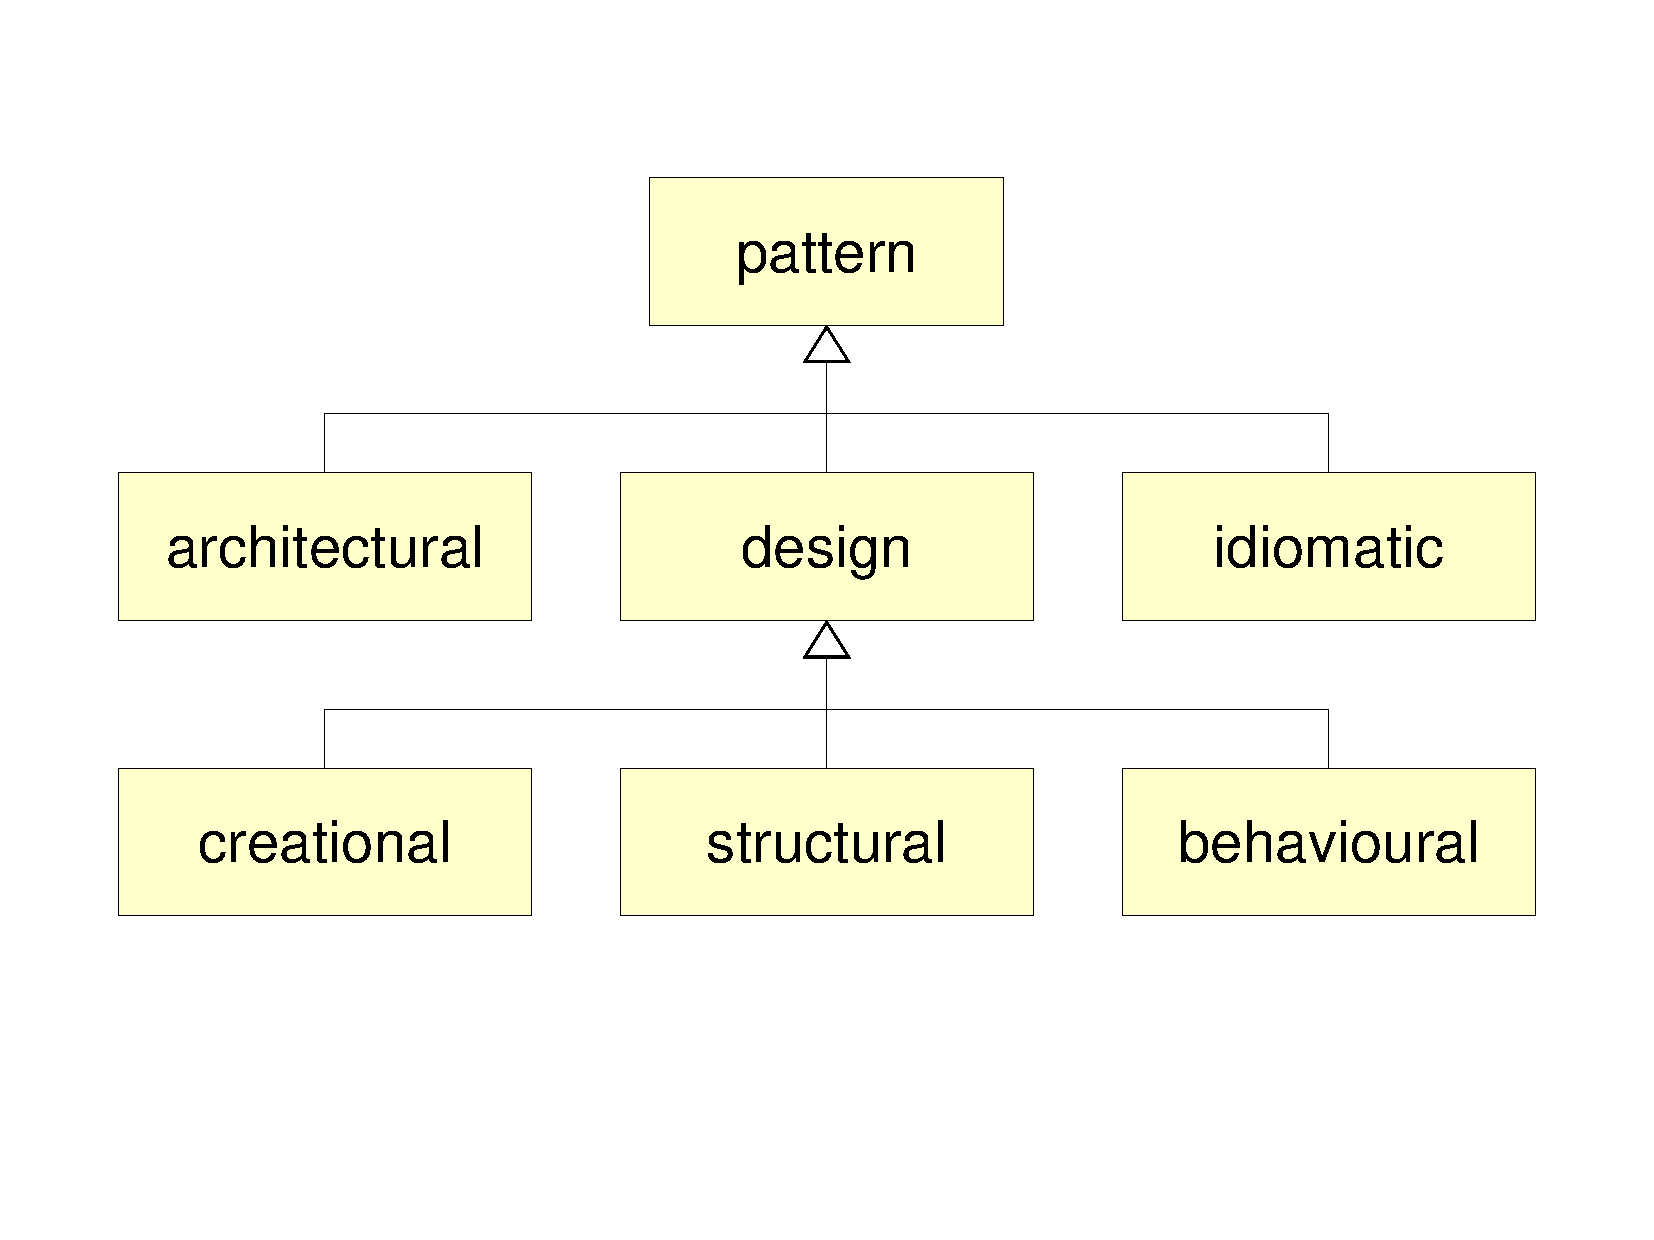
\includegraphics[scale=0.3,angle=-90]{graphic/pattern.pdf}
        \caption{Software Pattern Classification}
        \label{pattern_figure}
    \end{center}
\end{figure}

Several schemes of \emph{Pattern Classification} exist. One possible is shown in
figure \ref{pattern_figure}. Considering the level of abstraction (granularity),
it distinguishes between \emph{Architectural-}, \emph{Design-} and \emph{Idiomatic}
patterns \cite{buschmann}. Design patterns, in turn, are divided after their
functionality (problem category) into \emph{Creational-}, \emph{Structural-}
and \emph{Behavioural} patterns \cite{gamma1995}. The Wikipedia Encyclopedia
\cite{wikipedia} mentions three further problem categories: \emph{Fundamental-},
\emph{Concurrency-} and \emph{Real-time} patterns. Other criteria (dimensions) of
classification exist. Fowler introduces a completely different category which he
calls \emph{Analysis Patterns} \cite{fowler1997}. These are applicable early in the
software engineering process (chapter \ref{software_engineering_process_heading}).
And he defines patterns that are more often used for describing the modelling
\emph{Language} than the actual \emph{Models} as \emph{Meta Model Patterns}.

In the following sections, a greater number of known patterns will be described
briefly. They form the scientific basis for the ideas following in part
\ref{contribution_heading} of this work and some of them appear in a modified
form in the language and interpreter introduced in part \ref{proof_heading}.
Chapter \ref{knowledge_schema_heading} moreover introduces a new pattern
systematics for which it references common patterns as introduced here.
However, since the next sections do not want to copy the work accomplished by
the above-mentioned authors, they refer to the corresponding literaric source
for more detailed explanation.

%
% $RCSfile: architectural.tex,v $
%
% Copyright (c) 2004. Christian Heller. All rights reserved.
%
% No copying, altering, distribution or any other actions concerning this
% document, except after explicit permission by the author!
% At some later point in time, this document is planned to be put under
% the GNU FDL license. For now, _everything_ is _restricted_ by the author.
%
% http://www.cybop.net
% - Cybernetics Oriented Programming -
%
% http://www.resmedicinae.org
% - Information in Medicine -
%
% @author Christian Heller <christian.heller@tuxtax.de>
%

\subsubsection{Architectural}
\label{architectural_heading}

\emph{Architectural Patterns} are templates for the gross design of software
systems. They describe concrete software architectures and provide basic
structuring (modularization) principles.

%
% $RCSfile: layers.tex,v $
%
% Copyright (C) 2002-2008. Christian Heller.
%
% Permission is granted to copy, distribute and/or modify this document
% under the terms of the GNU Free Documentation License, Version 1.1 or
% any later version published by the Free Software Foundation; with no
% Invariant Sections, with no Front-Cover Texts and with no Back-Cover
% Texts. A copy of the license is included in the section entitled
% "GNU Free Documentation License".
%
% http://www.cybop.net
% - Cybernetics Oriented Programming -
%
% http://www.resmedicinae.org
% - Information in Medicine -
%
% Version: $Revision: 1.1 $ $Date: 2008-08-19 20:41:07 $ $Author: christian $
% Authors: Christian Heller <christian.heller@tuxtax.de>
%

\subsubsection{Layers}
\label{layers_heading}
\index{Layers Pattern}
\index{Presentation Layer}
\index{Domain Logic Layer}
\index{Business Logic Layer}
\index{Data Source Layer}
\index{ISO OSI Model Layers}
\index{Relaxed Layered System}

The \emph{Layers} pattern \cite{buschmann} is one of the most often used
principles to subdivide a system into logical levels. One variant was shown in
figure \ref{logical_figure}, at the beginning of this chapter. It contained the
three layers \emph{Presentation}, \emph{Domain Logic} and \emph{Data Source}. A
more general illustration can be seen in figure \ref{layers_figure}. It shows a
client using the functionality encapsulated in a layer. That top-most layer
delegates subtasks to lower-level layers which are specialised on solving them.
Another well-known example making use of this pattern is the \emph{ISO OSI}
model as introduced in section \ref{systems_interconnection_heading}.

\begin{figure}[ht]
    \begin{center}
        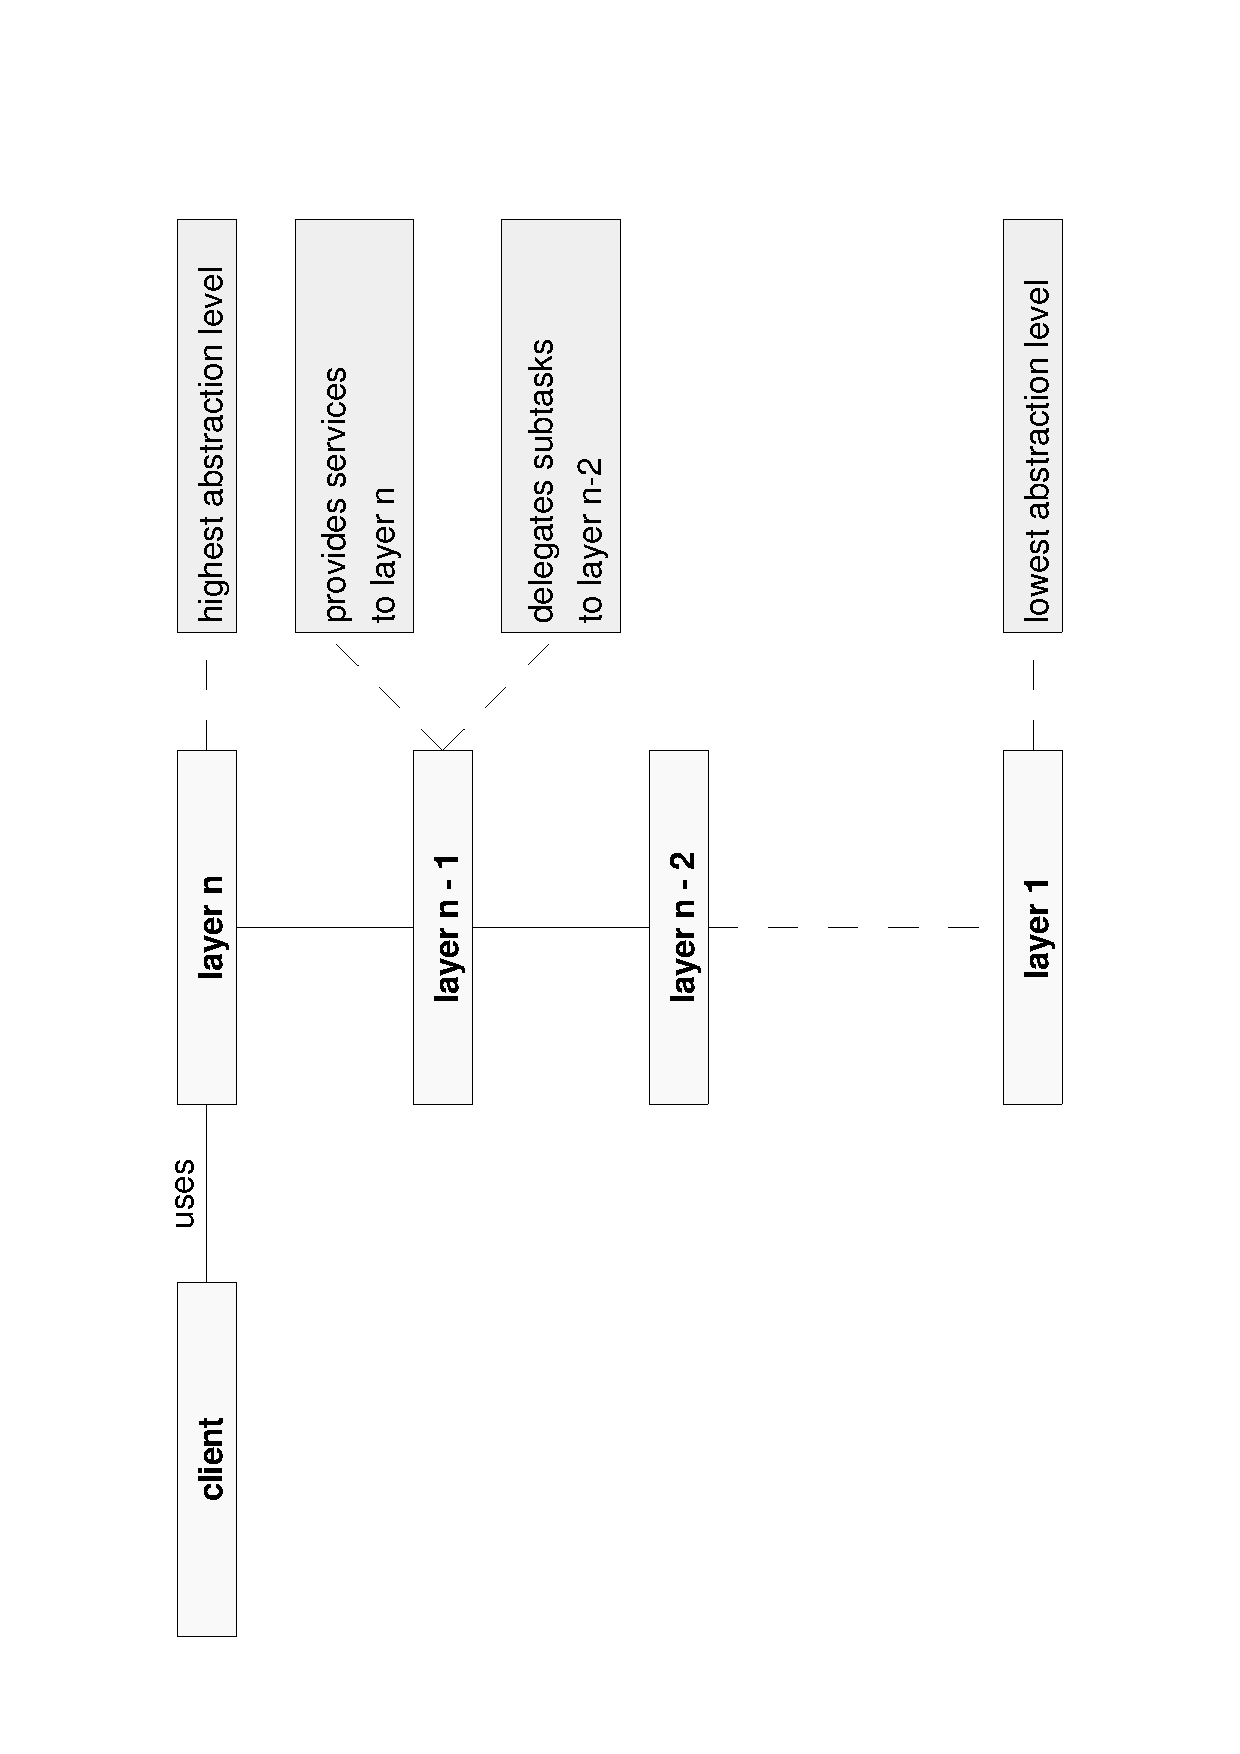
\includegraphics[scale=0.3,angle=-90]{graphic/layers.pdf}
        \caption{Layers Pattern}
        \label{layers_figure}
    \end{center}
\end{figure}

One variant of this pattern, mentioned by Buschmann \cite{buschmann}, is the
\emph{Relaxed-Layered-System}. It permits a layer to not only use the services
of its direct base layer, but also of yet lower-situated layers. The base layer,
in this case, is called \emph{transparent}.

The ontology examples in chapter \ref{knowledge_schema_heading} are organised
according to the \emph{Layers} pattern. Their layers represent levels of
growing granularity.

%
% $RCSfile: data_mapper.tex,v $
%
% Copyright (c) 2004. Christian Heller. All rights reserved.
%
% No copying, altering, distribution or any other actions concerning this
% document, except after explicit permission by the author!
% At some later point in time, this document is planned to be put under
% the GNU FDL license. For now, _everything_ is _restricted_ by the author.
%
% http://www.cybop.net
% - Cybernetics Oriented Programming -
%
% http://www.resmedicinae.org
% - Information in Medicine -
%
% @author Christian Heller <christian.heller@tuxtax.de>
%

\paragraph{Data Mapper}
\label{data_mapper_heading}

Besides the \emph{Domain Logic}, standard three-tier architectures contain a
\emph{Data Source} layer which may for example represent a database. Both layers
need to exchange data. Modern systems use OOP methods to implement the domain
model. Database models, on the other hand, are often implemented as
\emph{Entity Relationship Model} (ERM).

In order to avoid close coupling and a mix-up of both layers, the introduction
of an additional \emph{Data Mapper} layer \cite{fowler2002} in between the two
others may be justified (figure \ref{datamapper_figure}). The most important
idea of this pattern is to abolish the interdependencies of domain- and
persistence model (database).

\begin{figure}[ht]
    \begin{center}
        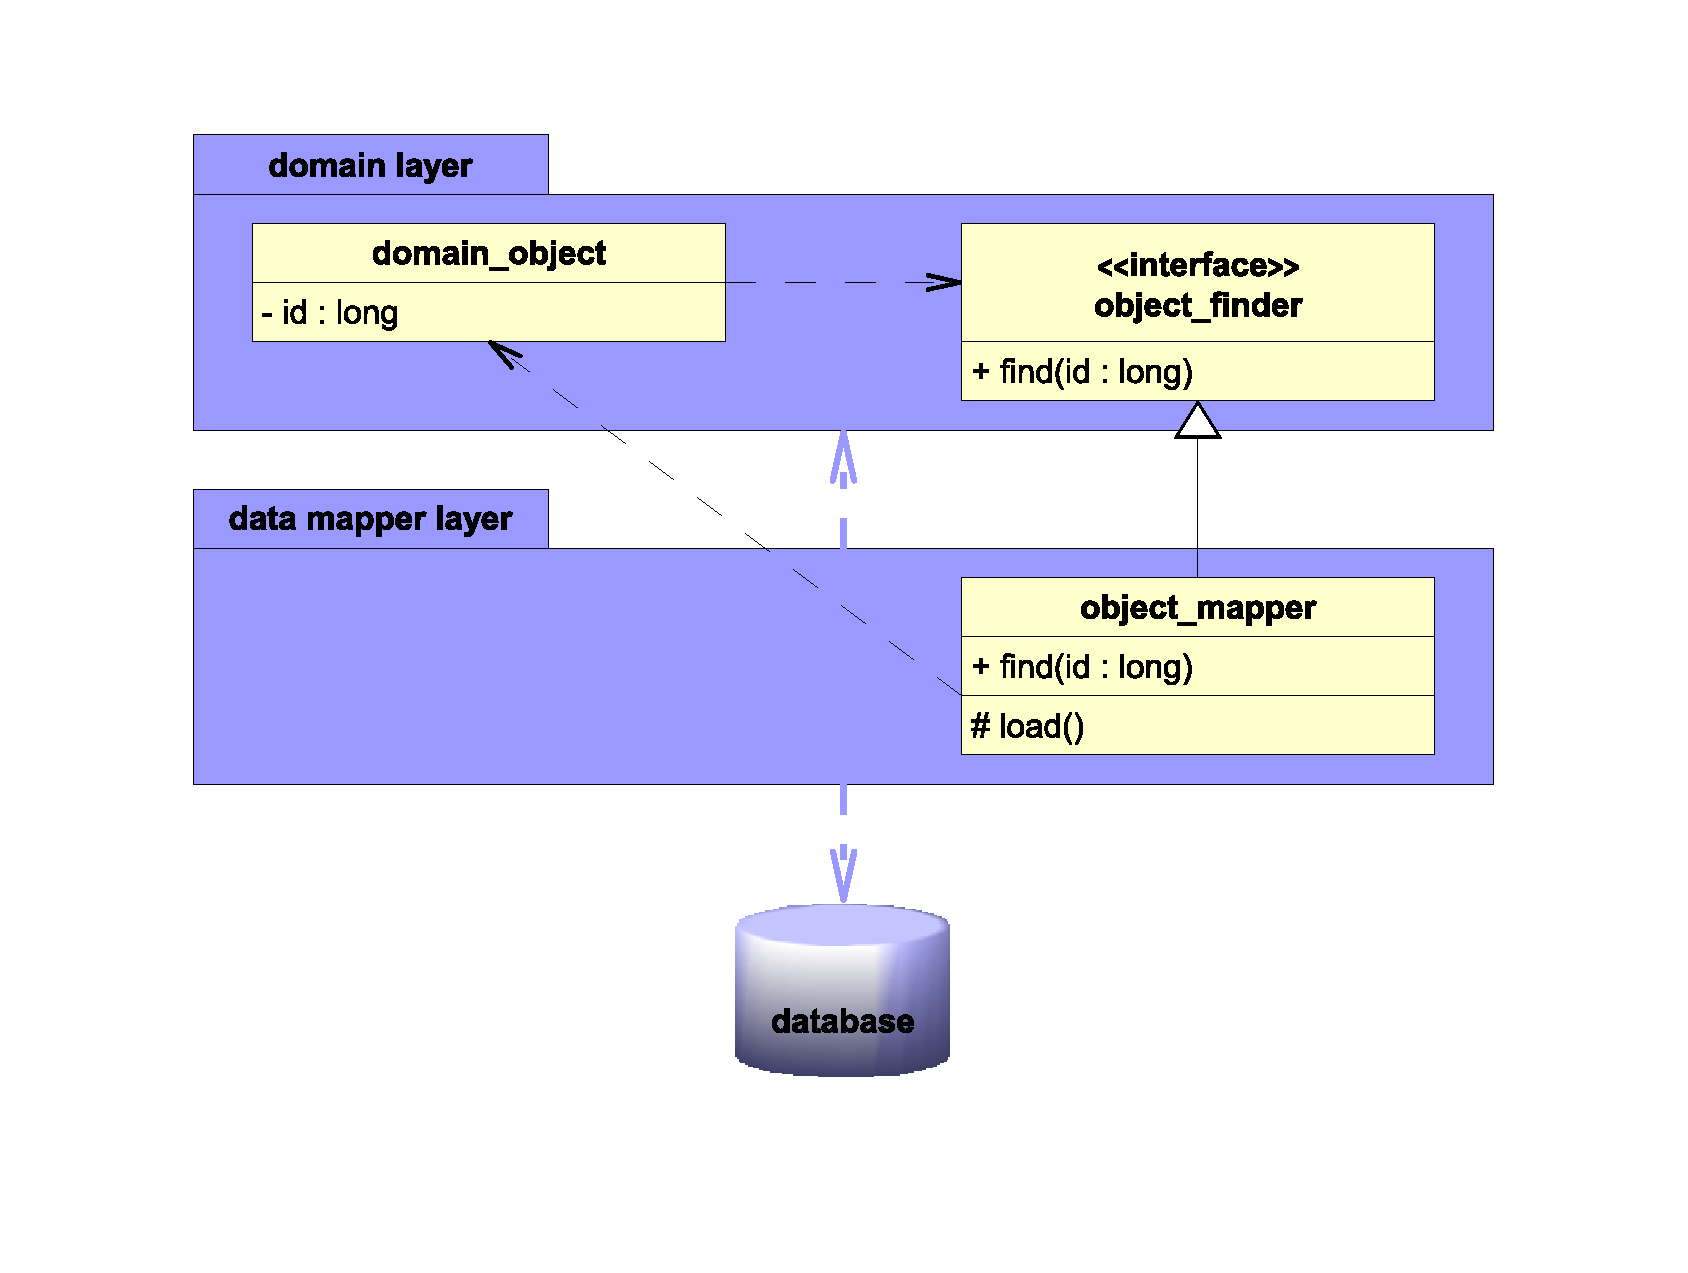
\includegraphics[scale=0.3]{vector/datamapper.eps}
        \caption{Data Mapper Pattern}
        \label{datamapper_figure}
    \end{center}
\end{figure}

The dashed arrows in figure \ref{datamapper_figure} indicate dependencies. The
data mapper layer knows the domain model- as well as the data source layer, via
\emph{unidirectional} relations. Its task is to \emph{translate} between the two,
in both directions. Domain model and data source know nothing from each other.

Each domain model class knows its appropriate interface (\emph{object\_finder})
but does not know the implementation of the same. That is, persistence- and
data retrieval mechanisms are hidden in front of the domain model. The
implementation (\emph{object\_mapper}) is part of the mapping package and also
implements all finder methods. It maps data of the received result sets to the
special attributes of the domain model objects.

The \emph{Mediator} pattern \cite{gamma1995} is similar to the \emph{Mapper}, in
that it is used to decouple different parts of a system. Fowler \cite{fowler2002}
writes: \textit{\ldots the objects that use a mediator are aware of it, even if
they aren't aware of each other; the objects that a mapper separates aren't even
aware of the mapper.}

Although the \emph{Data Mapper} pattern is very helpful at implementing OO
systems, two things are to be criticised:

Firstly, since the \emph{object\_finder} relies on functionality specific to the
retrieval of persistent data, it does actually belong into the data mapper layer
what, if done, would create bidirectional dependencies between the domain model-
and data mapper layer. But also with the \emph{object\_finder} remaining in the
domain model layer, dependencies are not purely unidirectional. It is true that
from an OO view, they are. Internally, however, a super class or interface
relates to its inheriting classes, so that it can call their methods to satisfy
the polymorphic behaviour.

Secondly, the layers do not truely build on each other. Taken a standard
architecture consisting of the following five -- instead of only three -- layers:

\begin{enumerate}
    \item Presentation
    \item Application Process
    \item Domain Model
    \item Data Mapper
    \item Data Source
\end{enumerate}

\ldots the application process does not only access the domain model layer, it
also has to manage (create and destroy) the objects of the data mapper layer.
In other words, it surpasses (disregards) the domain model layer when accessing
the data mapper layer directly.

%
% $RCSfile: data_transfer_object.tex,v $
%
% Copyright (C) 2002-2008. Christian Heller.
%
% Permission is granted to copy, distribute and/or modify this document
% under the terms of the GNU Free Documentation License, Version 1.1 or
% any later version published by the Free Software Foundation; with no
% Invariant Sections, with no Front-Cover Texts and with no Back-Cover
% Texts. A copy of the license is included in the section entitled
% "GNU Free Documentation License".
%
% http://www.cybop.net
% - Cybernetics Oriented Programming -
%
% http://www.resmedicinae.org
% - Information in Medicine -
%
% Version: $Revision: 1.1 $ $Date: 2008-08-19 20:41:06 $ $Author: christian $
% Authors: Christian Heller <christian.heller@tuxtax.de>
%

\subsubsection{Data Transfer Object}
\label{data_transfer_object_heading}
\index{Data Transfer Object Pattern}
\index{DTO}
\index{Assembler Object}
\index{Flat Data Structure}
\index{Translator Architecture}

\begin{figure}[ht]
    \begin{center}
       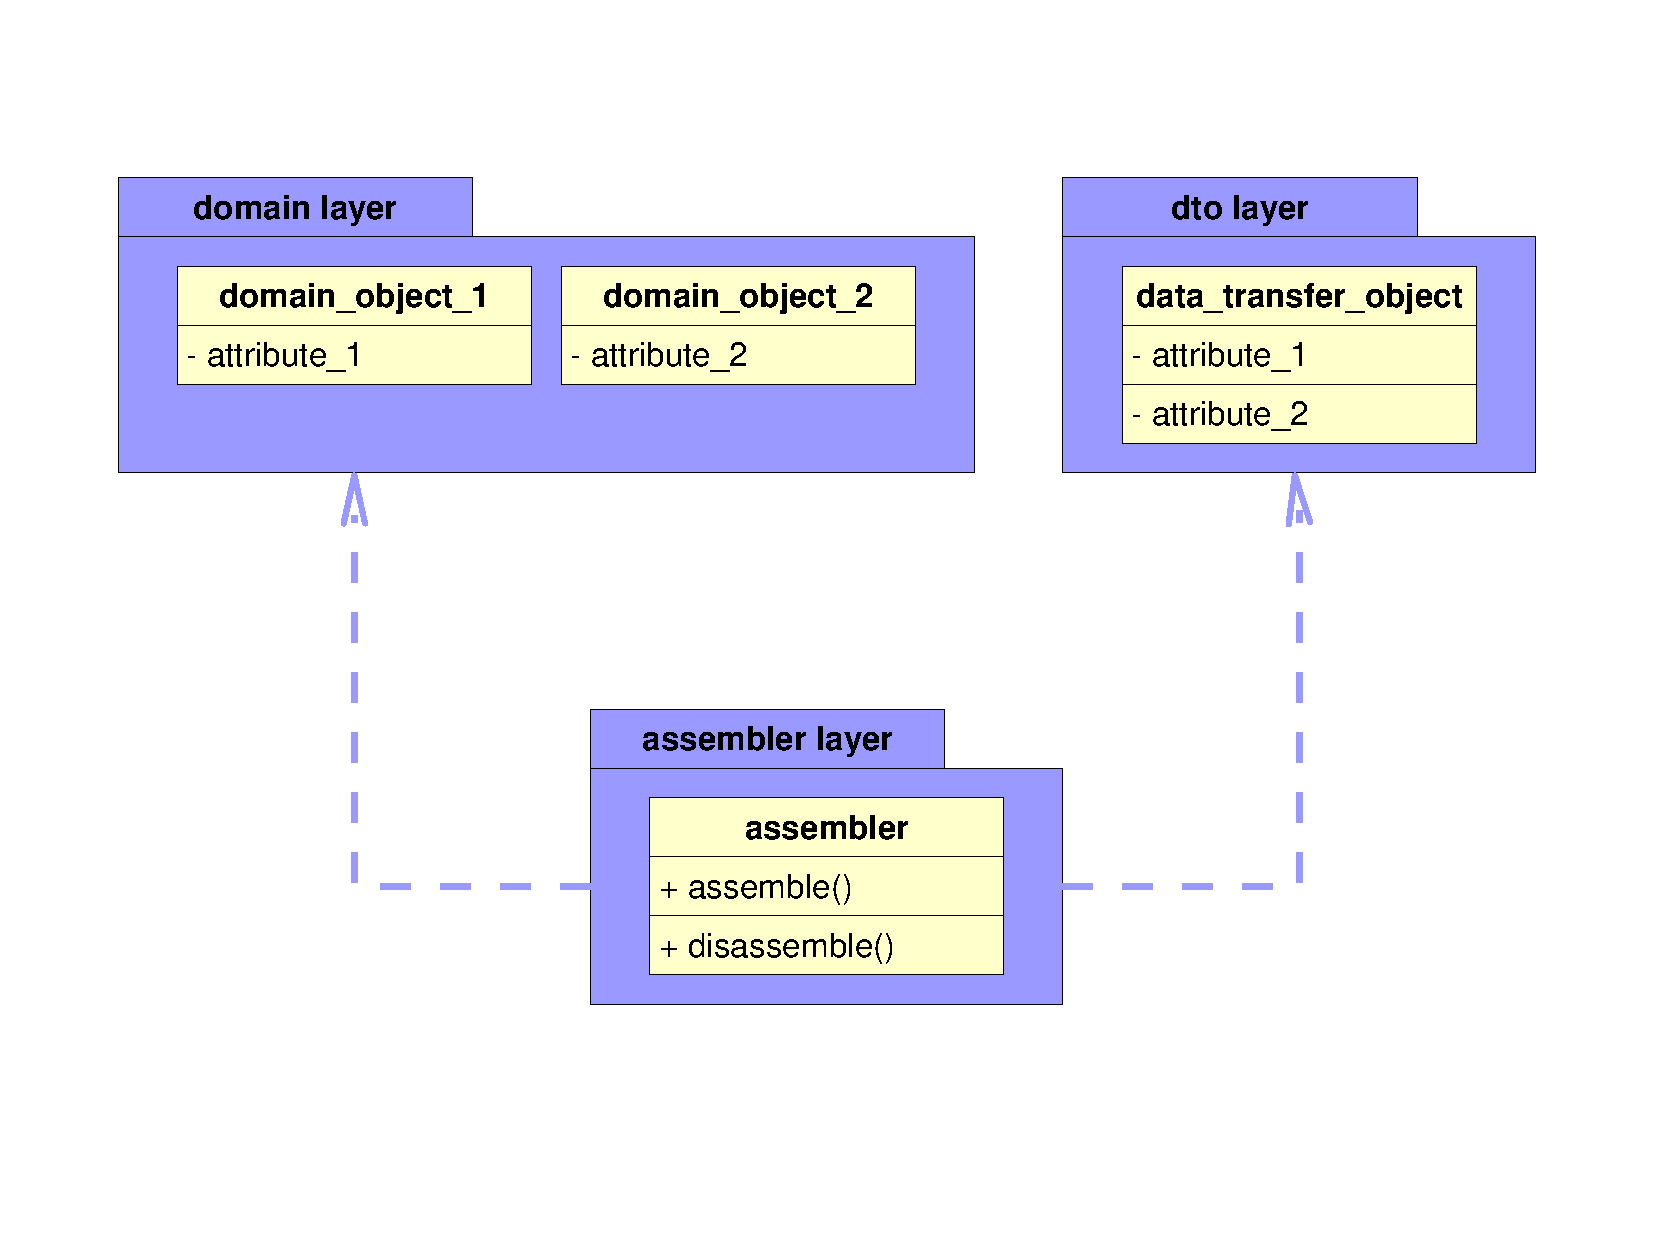
\includegraphics[scale=0.3,angle=-90]{graphic/dto.pdf}
       \caption{Data Transfer Object Pattern}
       \label{dto_figure}
    \end{center}
\end{figure}

It is a well-known fact that many small requests between two processes, and
even more between two hosts in a network need a lot of time. A local machine
with two processes has to permanently change the \emph{Program Context}; a
network has a lot of \emph{Transfers}. For each request, there is a necessity
of at least \emph{two} transfers -- the \emph{Question} of the client and the
\emph{Answer} of the server. Transfer methods are often expected to deliver
common data such as a Person's address, that is surname, first name, street,
zip-code, town and so on. These information is best retrieved by only
\emph{one} transfer call. That way, the client has to wait only once for a
server response and the server does not get too many single tasks. All address
data (in this example) would best be packaged together and sent back to the
client.

A scenario of that kind is exactly what the \emph{Data Transfer Object} pattern
\cite{fowler2002} proposes a solution for: A central \emph{Assembler} object
takes all common data of the server's domain model objects and assembles them
together into a special \emph{Data Transfer Object} (DTO), which is a flat data
structure (figure \ref{dto_figure}). The server will then send this DTO over
network to the client. On the client's side, a similar assembler takes the DTO,
finds out all received data and maps (disassembles) them to the client's domain
model. In that manner, a DTO is able to drastically improve the communication
performance.

Both, \emph{Data Mapper-} and DTO pattern translate one model into another. Due
to this similarity, chapter \ref{state_and_logic_heading} will try to merge
them into a common \emph{Translator} architecture.

%
% $RCSfile: model_view_controller.tex,v $
%
% Copyright (C) 2002-2008. Christian Heller.
%
% Permission is granted to copy, distribute and/or modify this document
% under the terms of the GNU Free Documentation License, Version 1.1 or
% any later version published by the Free Software Foundation; with no
% Invariant Sections, with no Front-Cover Texts and with no Back-Cover
% Texts. A copy of the license is included in the section entitled
% "GNU Free Documentation License".
%
% http://www.cybop.net
% - Cybernetics Oriented Programming -
%
% http://www.resmedicinae.org
% - Information in Medicine -
%
% Version: $Revision: 1.1 $ $Date: 2008-08-19 20:41:07 $ $Author: christian $
% Authors: Christian Heller <christian.heller@tuxtax.de>
%

\subsubsection{Model View Controller}
\label{model_view_controller_heading}
\index{Model View Controller Pattern}
\index{MVC}
\index{Graphical User Interface}
\index{GUI}
\index{Observer Pattern}
\index{Strategy Pattern}
\index{Wrapper Pattern}
\index{Composite Pattern}
\index{Java Foundation Classes}
\index{JFC}
\index{Microsoft Foundation Classes}
\index{MFC}
\index{Document View MVC Variant}
\index{Translator Architecture}

After having had a closer look at design patterns for persistence
(\emph{Data Mapper}) and communication (\emph{Data Transfer Object}), this
section considers the presentation layer of an application (figure
\ref{logical_figure}), which is often realised in form of a
\emph{Graphical User Interface} (GUI). Nowadays, the well-known
\emph{Model View Controller} (MVC) pattern \cite{buschmann, fowler2002} is used
by a majority of standard business applications. Its principle is to have the
\emph{Model} holding domain data, the \emph{View} accessing and displaying
these data and the \emph{Controller} providing the workflow of the application
by handling any action events happening on the view (figure \ref{mvc_figure}).
This separation eases the creation of applications with many synchronous views
on the same data. Internally, the MVC may consist of design patterns like:

\begin{figure}[ht]
    \begin{center}
        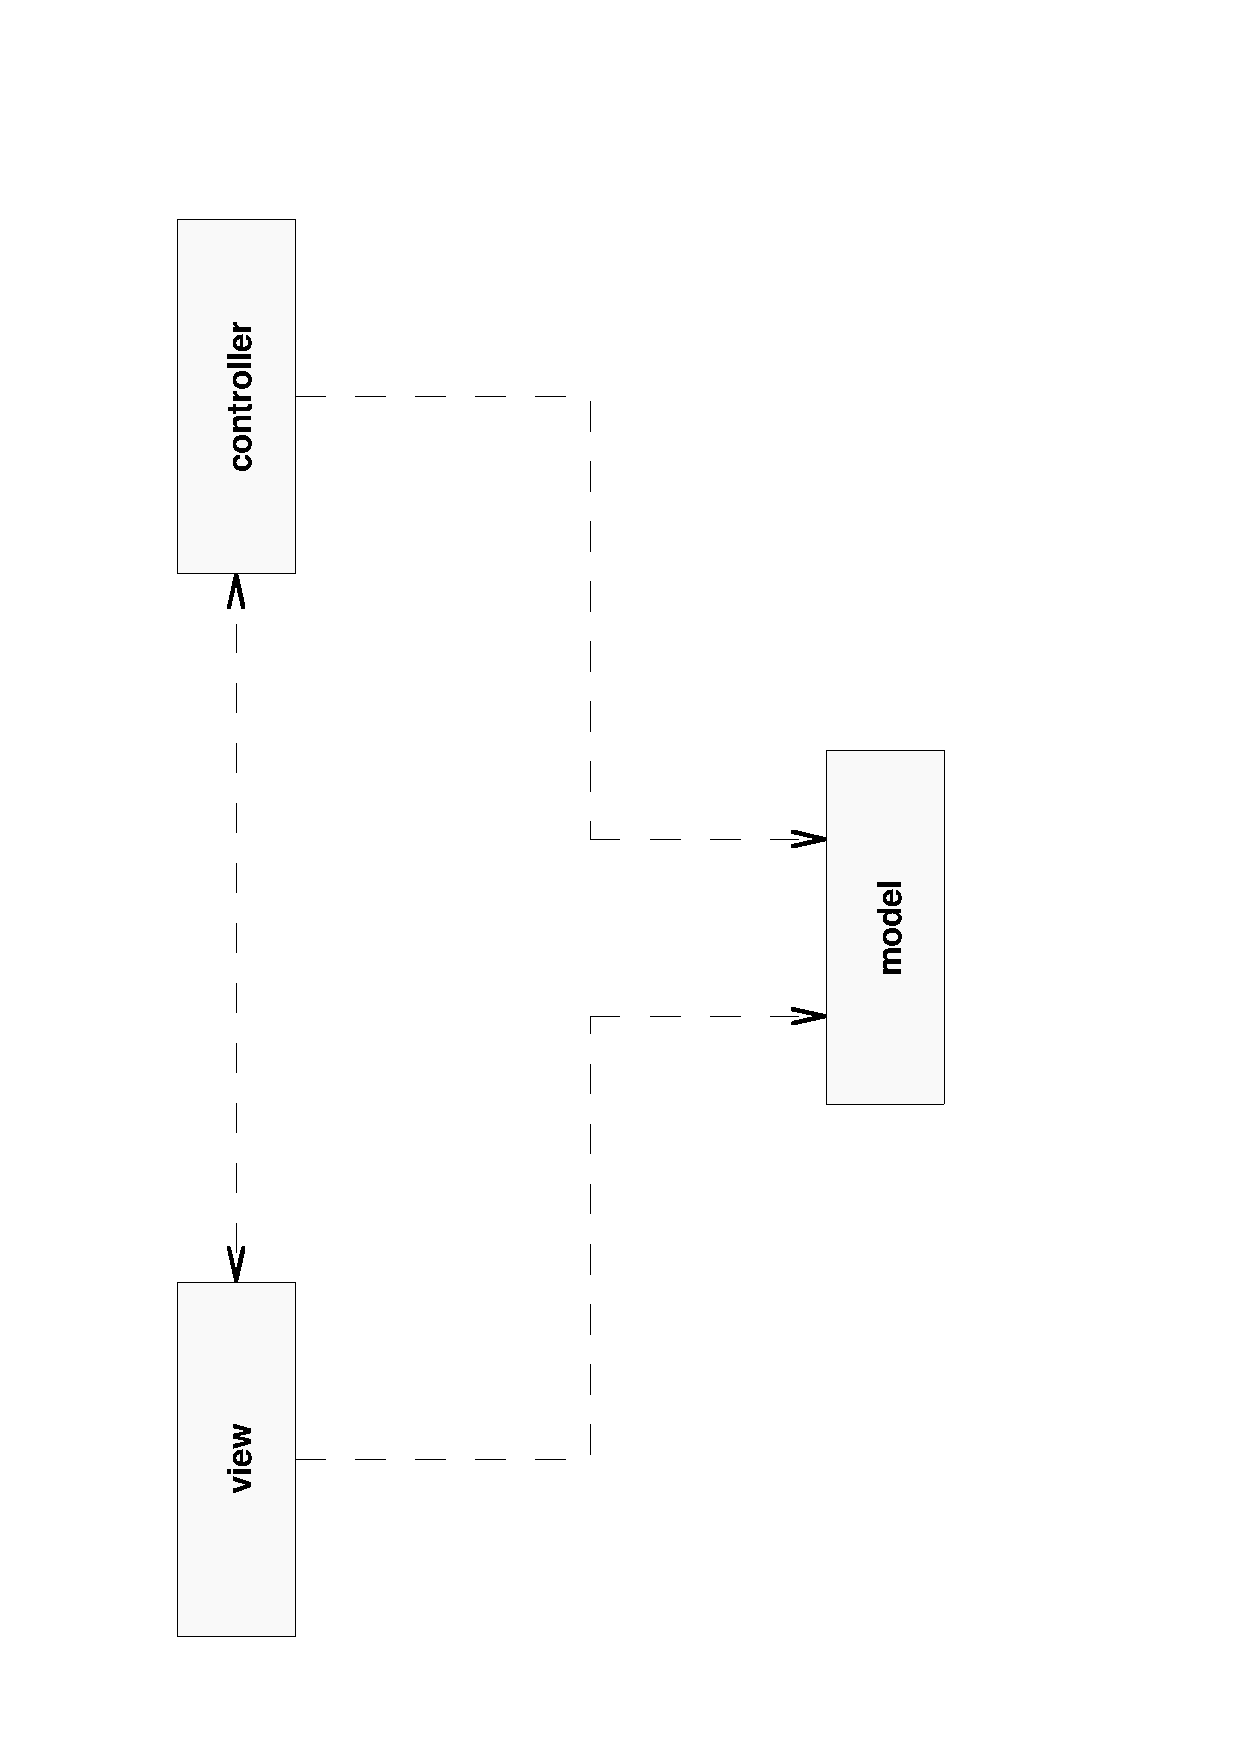
\includegraphics[scale=0.3,angle=-90]{graphic/mvc.pdf}
        \caption{Model View Controller Pattern}
        \label{mvc_figure}
    \end{center}
\end{figure}

\begin{itemize}
    \item[-] \emph{Observer} (section \ref{observer_heading}) which notifies
        the views about data model changes
    \item[-] \emph{Strategy} \cite{gamma1995} which encapsulates exchangeable
        functionality of the controller
    \item[-] \emph{Wrapper} (section \ref{wrapper_heading}) which delegates
        controller functionality to the \emph{Strategy}
    \item[-] \emph{Composite} (section \ref{composite_heading}) which equips
        graphical views with a hierarchical structure
\end{itemize}

Some MVC implementations like parts of the \emph{Java Foundation Classes} (JFC)
use a simplified version not separating controllers from their views. The
\emph{Microsoft Foundation Classes} (MFC) C++ library calls its implementation
\emph{Document-View}.

Besides the above-mentioned patterns \emph{Data Mapper} and DTO, MVC is the
third one getting merged into a common \emph{Translator} architecture, in
chapter \ref{state_and_logic_heading}.

%
% $RCSfile: hierarchical_model_view_controller.tex,v $
%
% Copyright (C) 2002-2008. Christian Heller.
%
% Permission is granted to copy, distribute and/or modify this document
% under the terms of the GNU Free Documentation License, Version 1.1 or
% any later version published by the Free Software Foundation; with no
% Invariant Sections, with no Front-Cover Texts and with no Back-Cover
% Texts. A copy of the license is included in the section entitled
% "GNU Free Documentation License".
%
% http://www.cybop.net
% - Cybernetics Oriented Programming -
%
% http://www.resmedicinae.org
% - Information in Medicine -
%
% Version: $Revision: 1.1 $ $Date: 2008-08-19 20:41:07 $ $Author: christian $
% Authors: Christian Heller <christian.heller@tuxtax.de>
%

\subsubsection{Hierarchical Model View Controller}
\label{hierarchical_model_view_controller_heading}
\index{Hierarchical Model View Controller Pattern}
\index{HMVC}
\index{Model View Controller Pattern}
\index{MVC}
\index{Composite Pattern}
\index{Layers Pattern}
\index{Chain of Responsibility Pattern}
\index{Presentation Layer}
\index{MVC Triad}
\index{Presentation Abstraction Control}
\index{PAC}
\index{PAC Agent}

There exist several extensions of the MVC pattern, one of them being the
\emph{Hierarchical Model View Controller} (HMVC) \cite{cai}. It combines the
patterns \emph{Composite} (section \ref{composite_heading}), \emph{Layers}
(section \ref{layers_heading}) and \emph{Chain of Responsibility} (section
\ref{chain_of_responsibility_heading}) into one conceptual architecture (figure
\ref{hmvc_figure}). This architecture divides the presentation layer into
hierarchical sections containing so-called \emph{MVC Triads}. The triads
conventionally consist of \emph{Model}, \emph{View} and \emph{Controller},
each. They communicate with each other by relating over their controller
object. Following the \emph{Layers} pattern, only neighbouring layers know from
each other.

\begin{figure}[ht]
    \begin{center}
        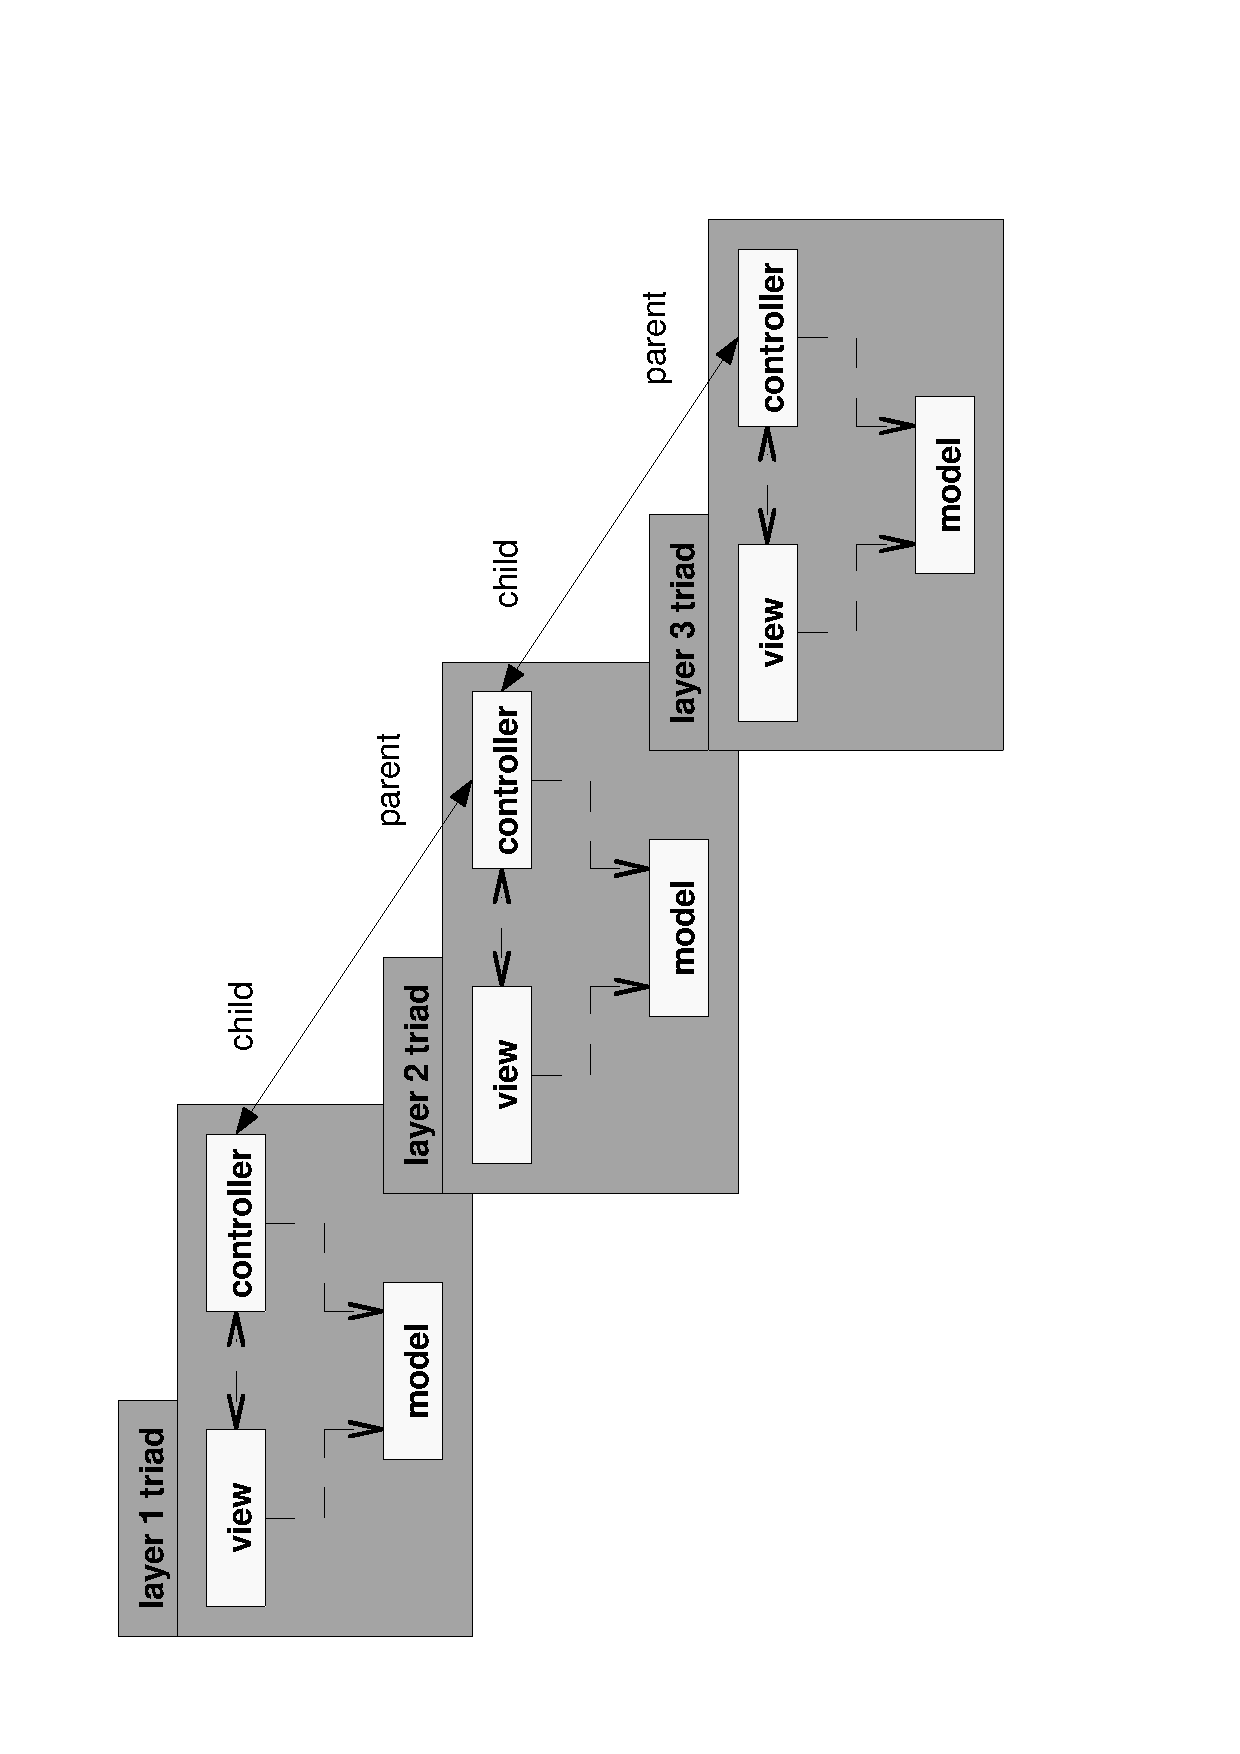
\includegraphics[scale=0.3,angle=-90]{graphic/hmvc.pdf}
        \caption{Hierarchical Model View Controller Pattern}
        \label{hmvc_figure}
    \end{center}
\end{figure}

As a practical example, the upper-most triad could represent a graphical
\emph{Dialogue} and the next lower one a \emph{Panel}. Being a container, too,
the panel could hold a third triad like for example a \emph{Button}. Events
occuring at the button are then normally processed by the corresponding
controller belonging to the button's triad. If, however, the button controller
cannot handle the event, that is forwarded along the chain of responsibility to
the controller of the higher-next layer. If also the panel controller does not
know how to handle the event, the final responsibility falls to the controller
of the dialogue's triad.

The HMVC is similar to the \emph{Presentation Abstraction Control} (PAC) pattern
\cite{buschmann}. A \emph{PAC Agent} is comparable to an \emph{HMVC Triad}.

Chapter \ref{knowledge_schema_heading} will apply the principle of
\emph{Hierarchy} not only to logic- (controller), but also to user interface-
(view), domain- and further models.

%
% $RCSfile: microkernel.tex,v $
%
% Copyright (c) 2004. Christian Heller. All rights reserved.
%
% No copying, altering, distribution or any other actions concerning this
% document, except after explicit permission by the author!
% At some later point in time, this document is planned to be put under
% the GNU FDL license. For now, _everything_ is _restricted_ by the author.
%
% http://www.cybop.net
% - Cybernetics Oriented Programming -
%
% http://www.resmedicinae.org
% - Information in Medicine -
%
% @author Christian Heller <christian.heller@tuxtax.de>
%

\paragraph{Microkernel}
\label{microkernel_heading}

The \emph{Microkernel} pattern \cite{buschmann} allows to keep a system flexible
and adaptable to changing requirements or new technologies. A minimal functional
\emph{Kernel} gets separated from extended functionality. The kernel may call
internal- or external servers (figure \ref{microkernel_figure}) to let them
solve special tasks which do not belong to its own core responsibility. Internal
servers are often called \emph{Daemons}.

\begin{figure}[ht]
    \begin{center}
        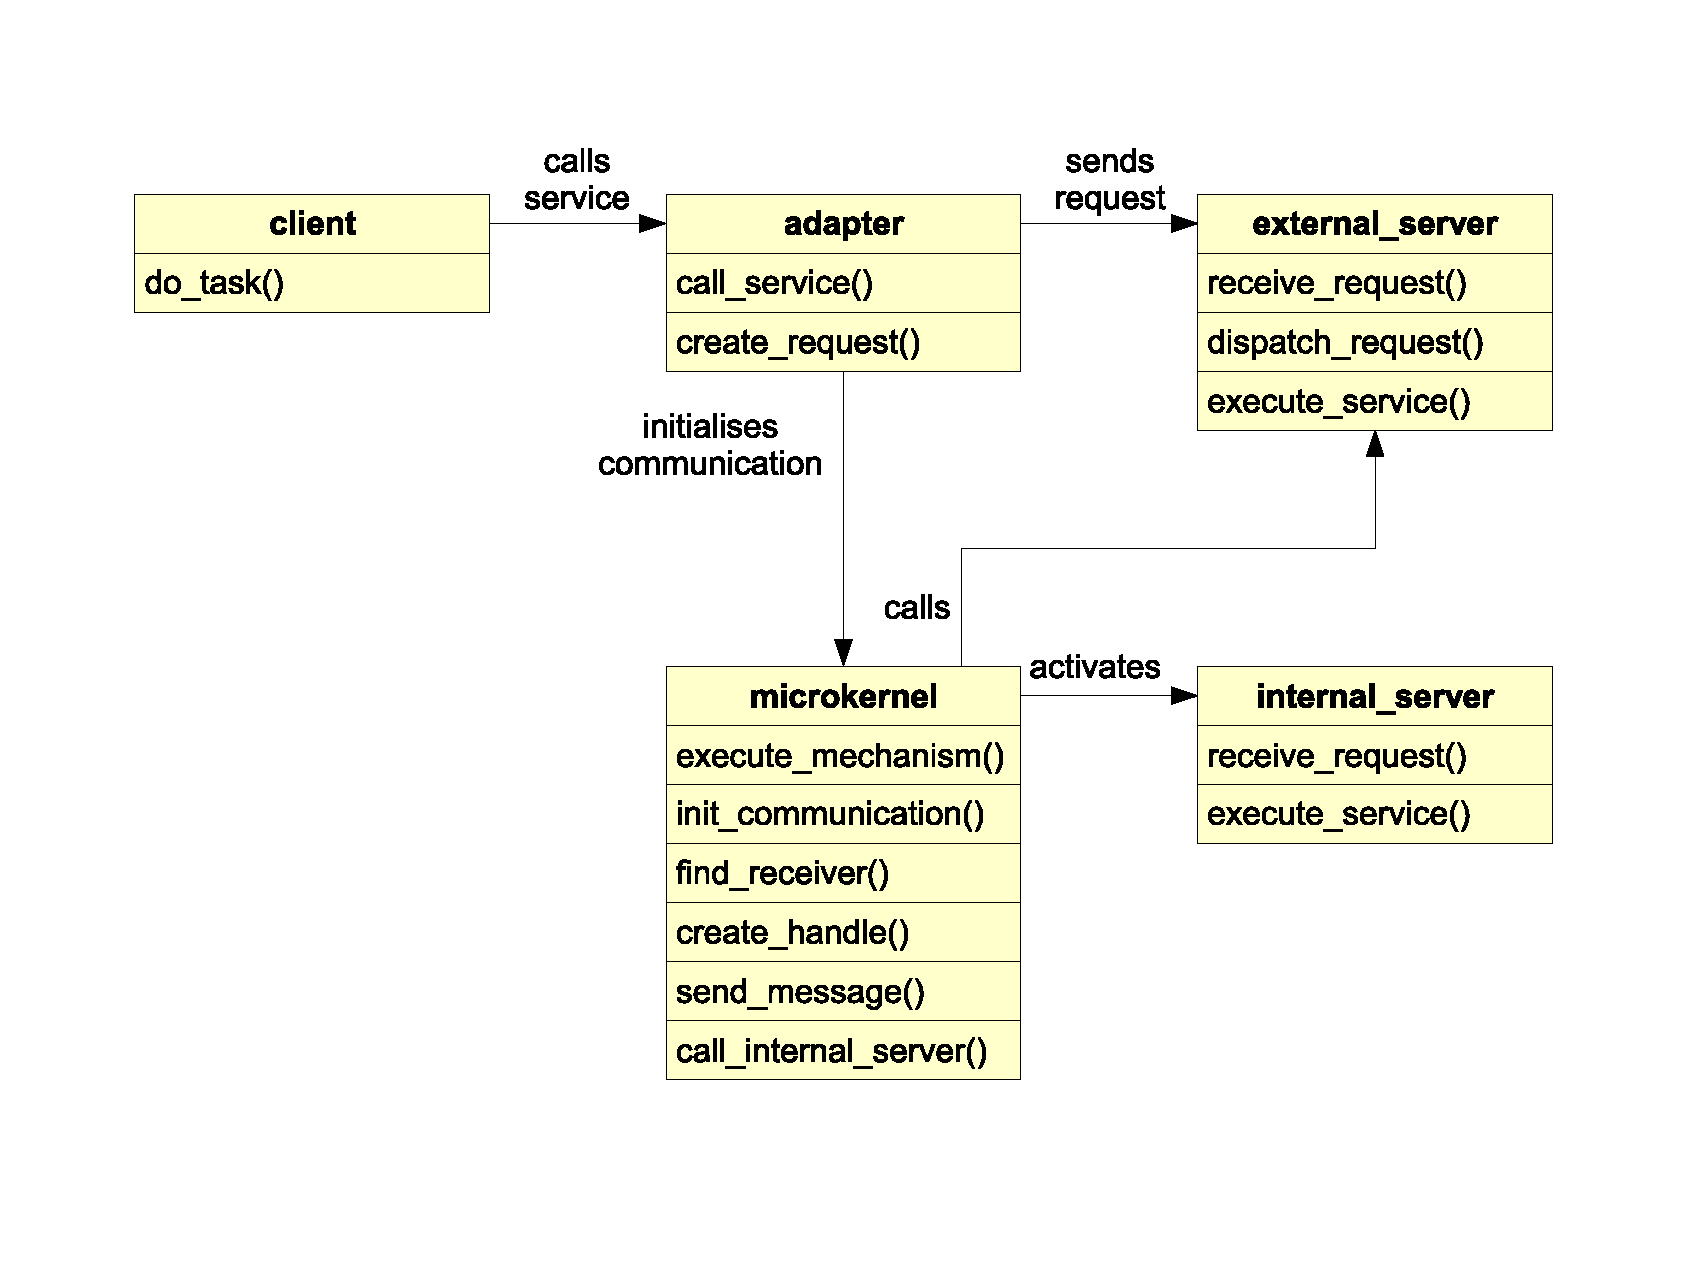
\includegraphics[scale=0.3]{vector/microkernel.eps}
        \caption{Microkernel Pattern}
        \label{microkernel_figure}
    \end{center}
\end{figure}

This pattern provides a \emph{Plug \& Play} environment and serves as base
architecture for many modern \emph{Operating Systems} (OS). Andrew S. Tanenbaum
recommends its use as well \cite{tanenbaum2001}.

%
% $RCSfile: broker.tex,v $
%
% Copyright (C) 2002-2008. Christian Heller.
%
% Permission is granted to copy, distribute and/or modify this document
% under the terms of the GNU Free Documentation License, Version 1.1 or
% any later version published by the Free Software Foundation; with no
% Invariant Sections, with no Front-Cover Texts and with no Back-Cover
% Texts. A copy of the license is included in the section entitled
% "GNU Free Documentation License".
%
% http://www.cybop.net
% - Cybernetics Oriented Programming -
%
% http://www.resmedicinae.org
% - Information in Medicine -
%
% Version: $Revision: 1.1 $ $Date: 2008-08-19 20:41:05 $ $Author: christian $
% Authors: Christian Heller <christian.heller@tuxtax.de>
%

\subsubsection{Broker}
\label{broker_heading}
\index{Broker Pattern}
\index{Distributed Application}

The \emph{Broker} pattern \cite{buschmann} may support the creation of an IT
infrastructure for distributed applications. It connects decoupled components
which interact through remote service invocations (figure \ref{broker_figure}).
The broker is responsible for coordinating all communication, for forwarding
requests as well as for transmitting results and exceptions.

%
% CAUTION! This file actually contains a graphics, which was moved to
% the 'microkernel.tex' file, for better formatting results in the document.
%

Chapter \ref{cybernetics_oriented_interpreter_heading} introduces an
interpreter program being able to act as broker.

%
% $RCSfile: pipes_and_filters.tex,v $
%
% Copyright (C) 2002-2008. Christian Heller.
%
% Permission is granted to copy, distribute and/or modify this document
% under the terms of the GNU Free Documentation License, Version 1.1 or
% any later version published by the Free Software Foundation; with no
% Invariant Sections, with no Front-Cover Texts and with no Back-Cover
% Texts. A copy of the license is included in the section entitled
% "GNU Free Documentation License".
%
% http://www.cybop.net
% - Cybernetics Oriented Programming -
%
% http://www.resmedicinae.org
% - Information in Medicine -
%
% Version: $Revision: 1.1 $ $Date: 2008-08-19 20:41:08 $ $Author: christian $
% Authors: Christian Heller <christian.heller@tuxtax.de>
%

\subsubsection{Pipes and Filters}
\label{pipes_and_filters_heading}
\index{Pipes and Filters Pattern}
\index{Push Scenario for Data Forwarding}
\index{Pull Scenario for Data Forwarding}
\index{Mixed Push-Pull-Pipeline Scenario for Data Forwarding}
\index{Independent Loops Scenario for Data Forwarding}

Systems that process streams of data may make use of the \emph{Pipes and Filters}
pattern \cite{buschmann}. It encapsulates every processing step in an own
\emph{Filter} component and forwards the data through channels which are called
\emph{Pipeline} (figure \ref{pipesfilters_figure}). The data forwarding can
follow various scenarios:

\begin{figure}[ht]
    \begin{center}
        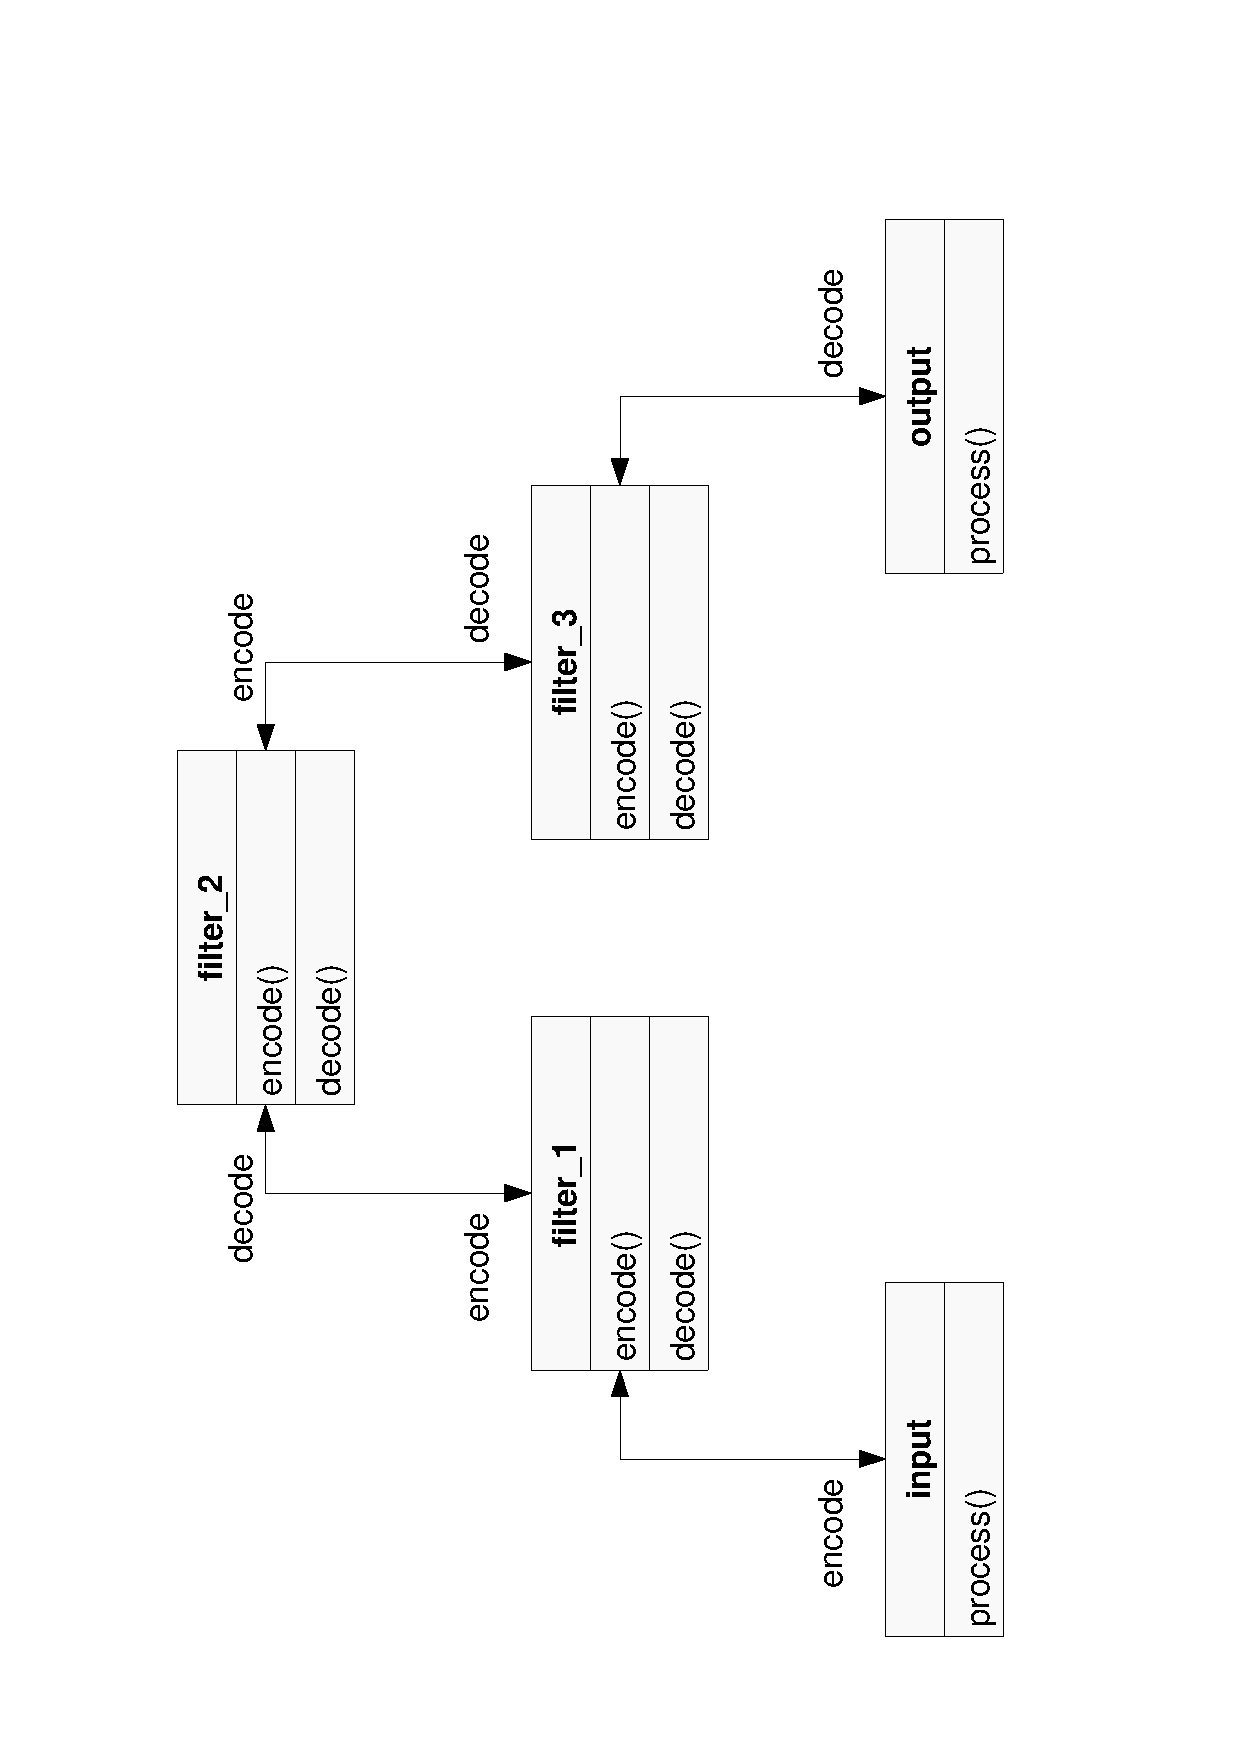
\includegraphics[scale=0.3,angle=-90]{graphic/pipesfilters.pdf}
        \caption{Pipes and Filters Pattern}
        \label{pipesfilters_figure}
    \end{center}
\end{figure}

\begin{itemize}
    \item[-] \emph{Push:} active filter pushes data to passive filter
    \item[-] \emph{Pull:} active filter pulls data from passive filter
    \item[-] \emph{Mixed Push-Pull-Pipeline:} all filters may push or pull data
    \item[-] \emph{Independent Loops:} all filters are active and access pipeline data
\end{itemize}

Families of related systems can be formed by changing the single filter
positions. Special communication filters are also used in the interpreter
program of chapter \ref{cybernetics_oriented_interpreter_heading}. Its filters
belong to neither of the above-listed forms of data forwarding, because they
are all passive, controlled from an outside entity which is not a filter
itself.

%
% $RCSfile: reflection.tex,v $
%
% Copyright (c) 2004. Christian Heller. All rights reserved.
%
% No copying, altering, distribution or any other actions concerning this
% document, except after explicit permission by the author!
% At some later point in time, this document is planned to be put under
% the GNU FDL license. For now, _everything_ is _restricted_ by the author.
%
% http://www.cybop.net
% - Cybernetics Oriented Programming -
%
% http://www.resmedicinae.org
% - Information in Medicine -
%
% @author Christian Heller <christian.heller@tuxtax.de>
%

\paragraph{Reflection}
\label{reflection_heading}

The \emph{Reflection} pattern \cite{buschmann} (also known under the synonyms
\emph{Open Implementation} or \emph{Meta-Level Architecture}) provides a
mechanism to change the structure and behaviour of a software system
\emph{dynamically}, that is at runtime, which is why that mechanism is sometimes
called \emph{Run Time Type Identification} (RTTI). A reflective system owns
information about itself and uses these to remain changeable and extensible.

\begin{figure}[ht]
    \begin{center}
        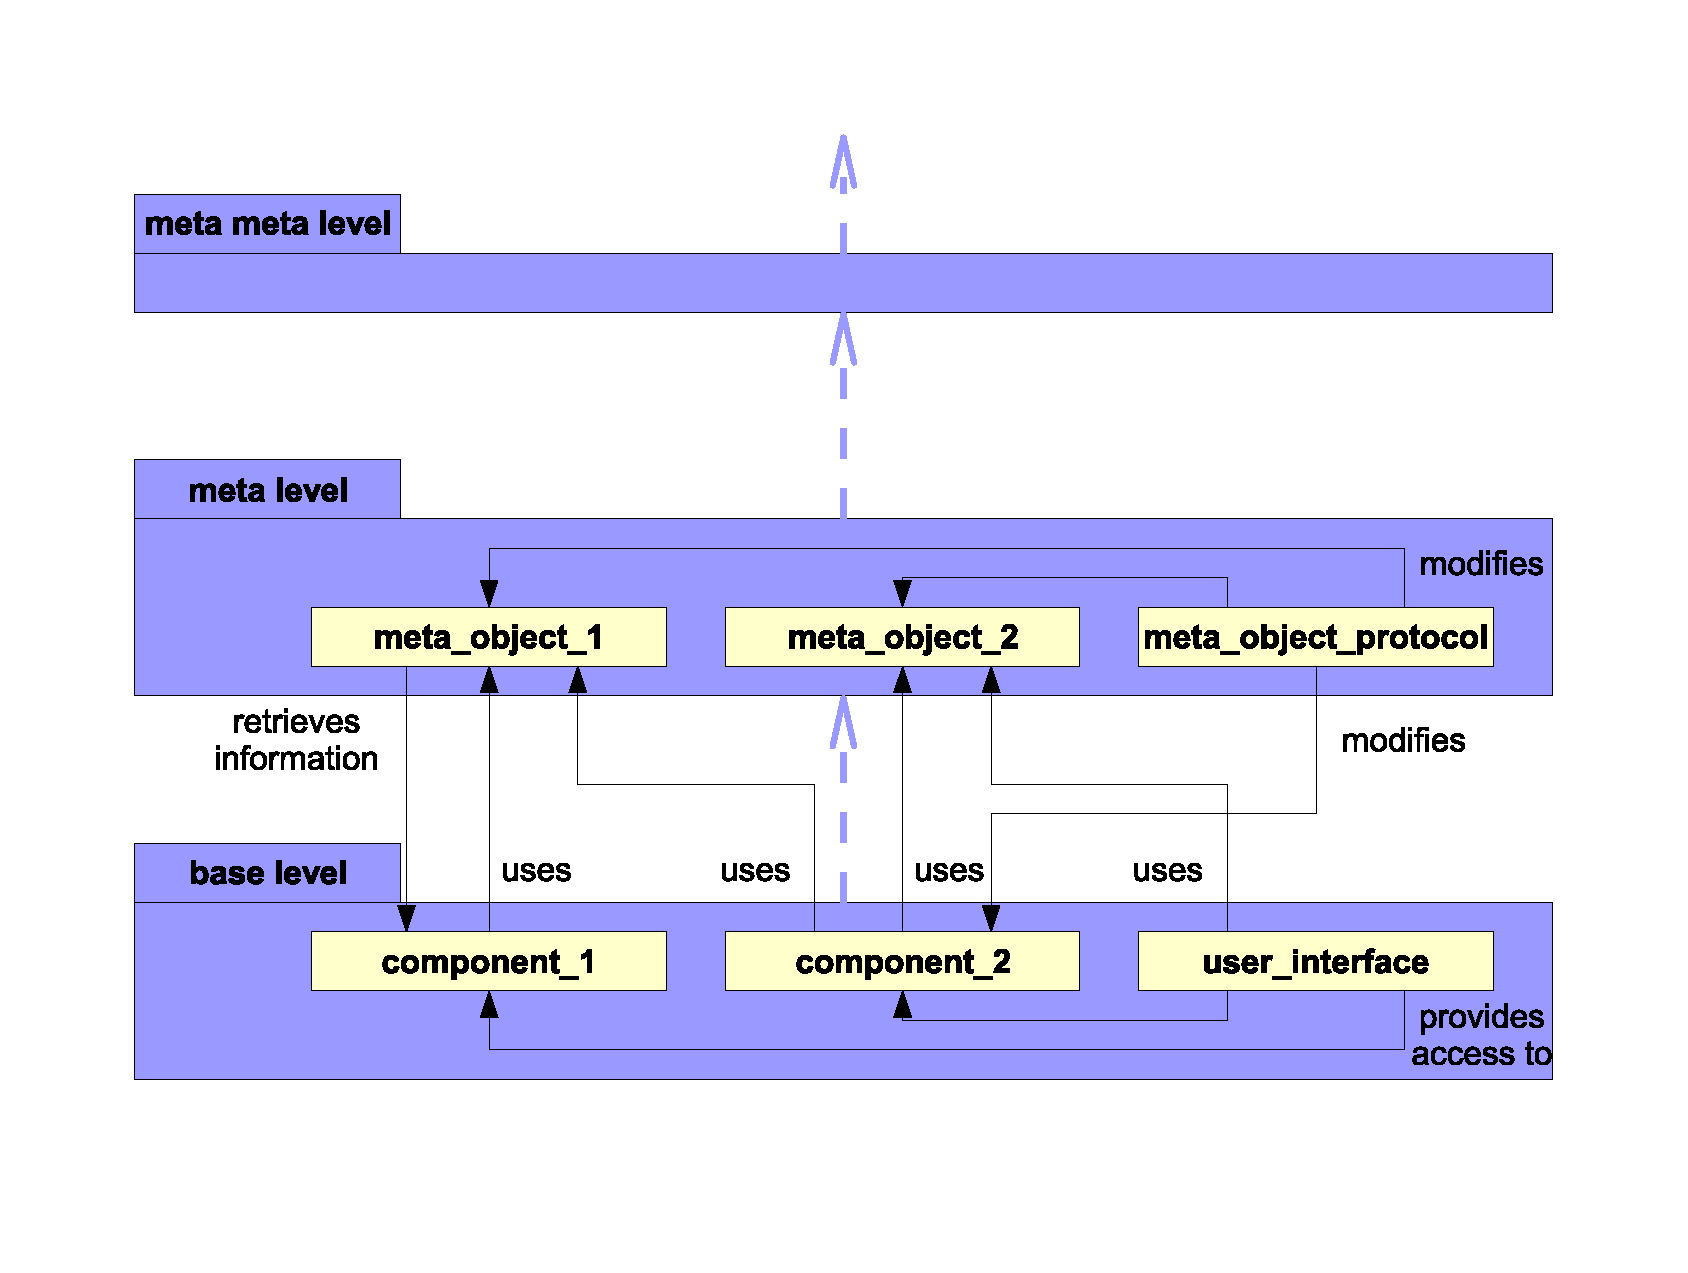
\includegraphics[scale=0.3]{vector/reflection.eps}
        \caption{Reflection Pattern}
        \label{reflection_figure}
    \end{center}
\end{figure}

Reflective information \emph{about} something is called \emph{Meta Information}.
Therefore, the level above the \emph{Base Level} in figure \ref{reflection_figure}
is labelled \emph{Meta Level}. The base level depends on the meta level, so that
changes in the meta level will also affect the base level. All manipulation of
meta objects happens through an interface called \emph{Meta Object Protocol}
(MOP), which is responsible for checking the correctness of- and for performing
a change. If a further level holds information about the meta level, then that
additional level is called \emph{Meta Meta Level}, and so forth.

Many examples of meta level architectures exist. In his book
\emph{Analysis Patterns} \cite{fowler1997}, Fowler uses them extensively.
He talks of \emph{Knowledge Level} (instead of meta level) and
\emph{Operational Level} (instead of base level). Elements of the
\emph{Unified Modeling Language} (UML) are defined in an own meta model
\cite{uml}. And the principles of reflection are also supported by several
programming languages, such as \emph{Smalltalk} \cite{smalltalk} and
\emph{Java} \cite{java}.

Classes (types) in a system have a static structure, as defined by the developer
at design time. Normally, most classes belong to the base level containing the
application logic. As written before, one way to change the structure and
behaviour of classes at runtime is to introduce a meta level providing type
information, in other words functionality that \emph{all} application classes
need. This helps avoid redundant implementations of the same functionality.

Looking closer at functionality, it turns out that some basic features like
persistence and communication occur repeatedly in almost all systems, while
other parts are specific to one concrete application. Traditionally, the
application classes in the base level have to cope with general system
functionality although that is not in their original interest. It therefore
seems logical to try to divide application- and system functionality, and to put
the latter into a meta level.


%
% $RCSfile: design.tex,v $
%
% Copyright (C) 2002-2008. Christian Heller.
%
% Permission is granted to copy, distribute and/or modify this document
% under the terms of the GNU Free Documentation License, Version 1.1 or
% any later version published by the Free Software Foundation; with no
% Invariant Sections, with no Front-Cover Texts and with no Back-Cover
% Texts. A copy of the license is included in the section entitled
% "GNU Free Documentation License".
%
% http://www.cybop.net
% - Cybernetics Oriented Programming -
%
% http://www.resmedicinae.org
% - Information in Medicine -
%
% Version: $Revision: 1.1 $ $Date: 2008-08-19 20:41:06 $ $Author: christian $
% Authors: Christian Heller <christian.heller@tuxtax.de>
%

\subsection{Design}
\label{design_heading}
\index{Design Pattern}

Gamma et al. \cite{gamma1995} define a design pattern as: \textit{description of
collaborating objects and classes which are taylored to solve a general design
problem in a special context.} Mostly, patterns are in relation to each other.
They can be combined to master more complex tasks.

%
% $RCSfile: command.tex,v $
%
% Copyright (c) 2004. Christian Heller. All rights reserved.
%
% No copying, altering, distribution or any other actions concerning this
% document, except after explicit permission by the author!
% At some later point in time, this document is planned to be put under
% the GNU FDL license. For now, _everything_ is _restricted_ by the author.
%
% http://www.cybop.net
% - Cybernetics Oriented Programming -
%
% http://www.resmedicinae.org
% - Information in Medicine -
%
% @author Christian Heller <christian.heller@tuxtax.de>
%

\paragraph{Command}
\label{command_heading}

The \emph{Command} pattern \cite{gamma1995}, also known as \emph{Action} or
\emph{Transaction}, sometimes also \emph{Signal}, encapsulates a command in
form of an object. That way, operations can get parameterised; they can be put
in a queue, be made undone or traced in a log book. Figure \ref{command_figure}
shows the structure of the pattern.

\begin{figure}[ht]
    \begin{center}
        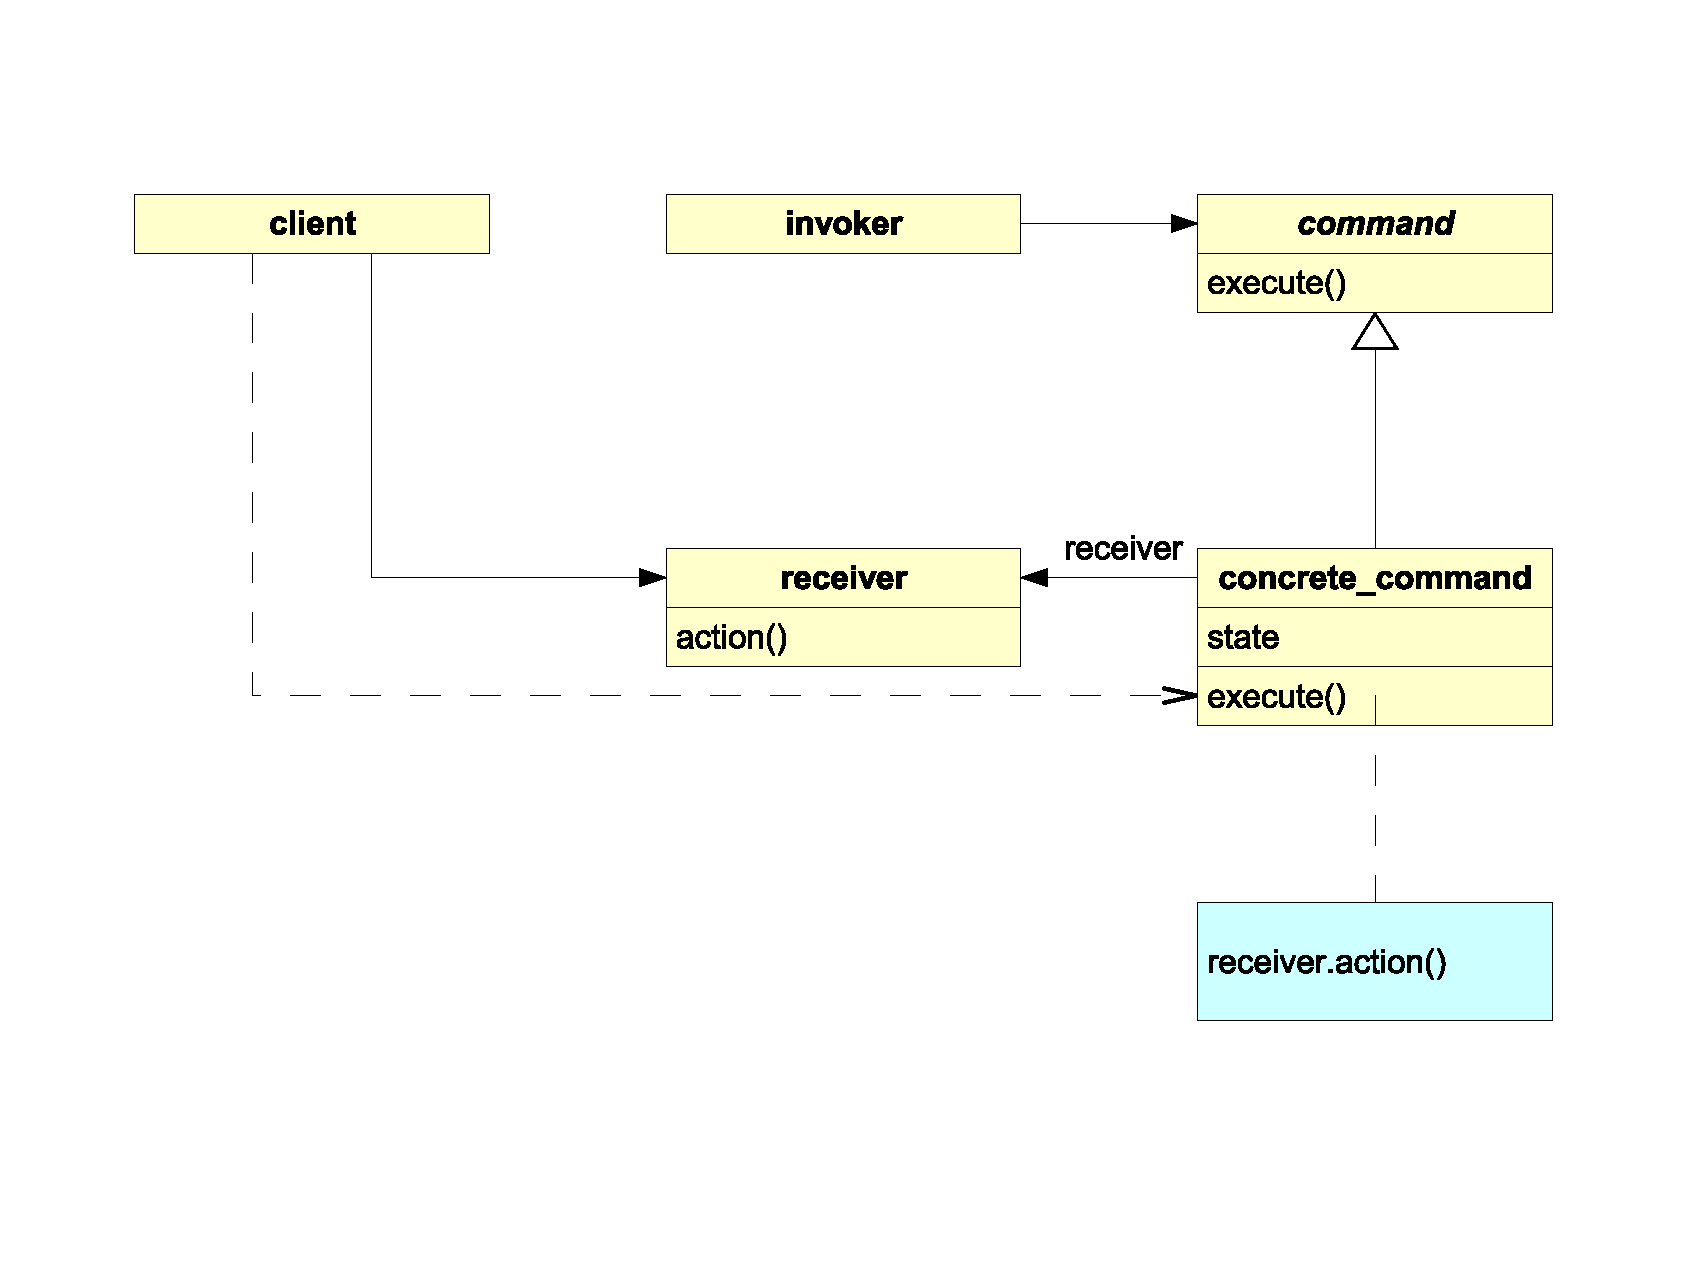
\includegraphics[scale=0.3]{vector/command.eps}
        \caption{Command Pattern}
        \label{command_figure}
    \end{center}
\end{figure}

%
% $RCSfile: wrapper.tex,v $
%
% Copyright (C) 2002-2008. Christian Heller.
%
% Permission is granted to copy, distribute and/or modify this document
% under the terms of the GNU Free Documentation License, Version 1.1 or
% any later version published by the Free Software Foundation; with no
% Invariant Sections, with no Front-Cover Texts and with no Back-Cover
% Texts. A copy of the license is included in the section entitled
% "GNU Free Documentation License".
%
% http://www.cybop.net
% - Cybernetics Oriented Programming -
%
% http://www.resmedicinae.org
% - Information in Medicine -
%
% Version: $Revision: 1.1 $ $Date: 2008-08-19 20:41:09 $ $Author: christian $
% Authors: Christian Heller <christian.heller@tuxtax.de>
%

\subsubsection{Wrapper}
\label{wrapper_heading}
\index{Wrapper Pattern}
\index{Adapter Pattern}
\index{Delegation Pattern}

The \emph{Wrapper} pattern \cite{gamma1995} allows otherwise incompatible
classes to work together. It can be seen as skin object enclosing (wrapping) an
inner core object, to which it provides access. In other words: It adapts the
interface of a class which is why Gamma et al. call the pattern \emph{Adapter}.
As can be seen in figure \ref{wrapper_figure}, this pattern makes heavy use of
\emph{Delegation}, where the \emph{Delegator} is the adapter (or wrapper) and
the \emph{Delegatee} is the class being adapted \cite{portland}.

\begin{figure}[ht]
    \begin{center}
        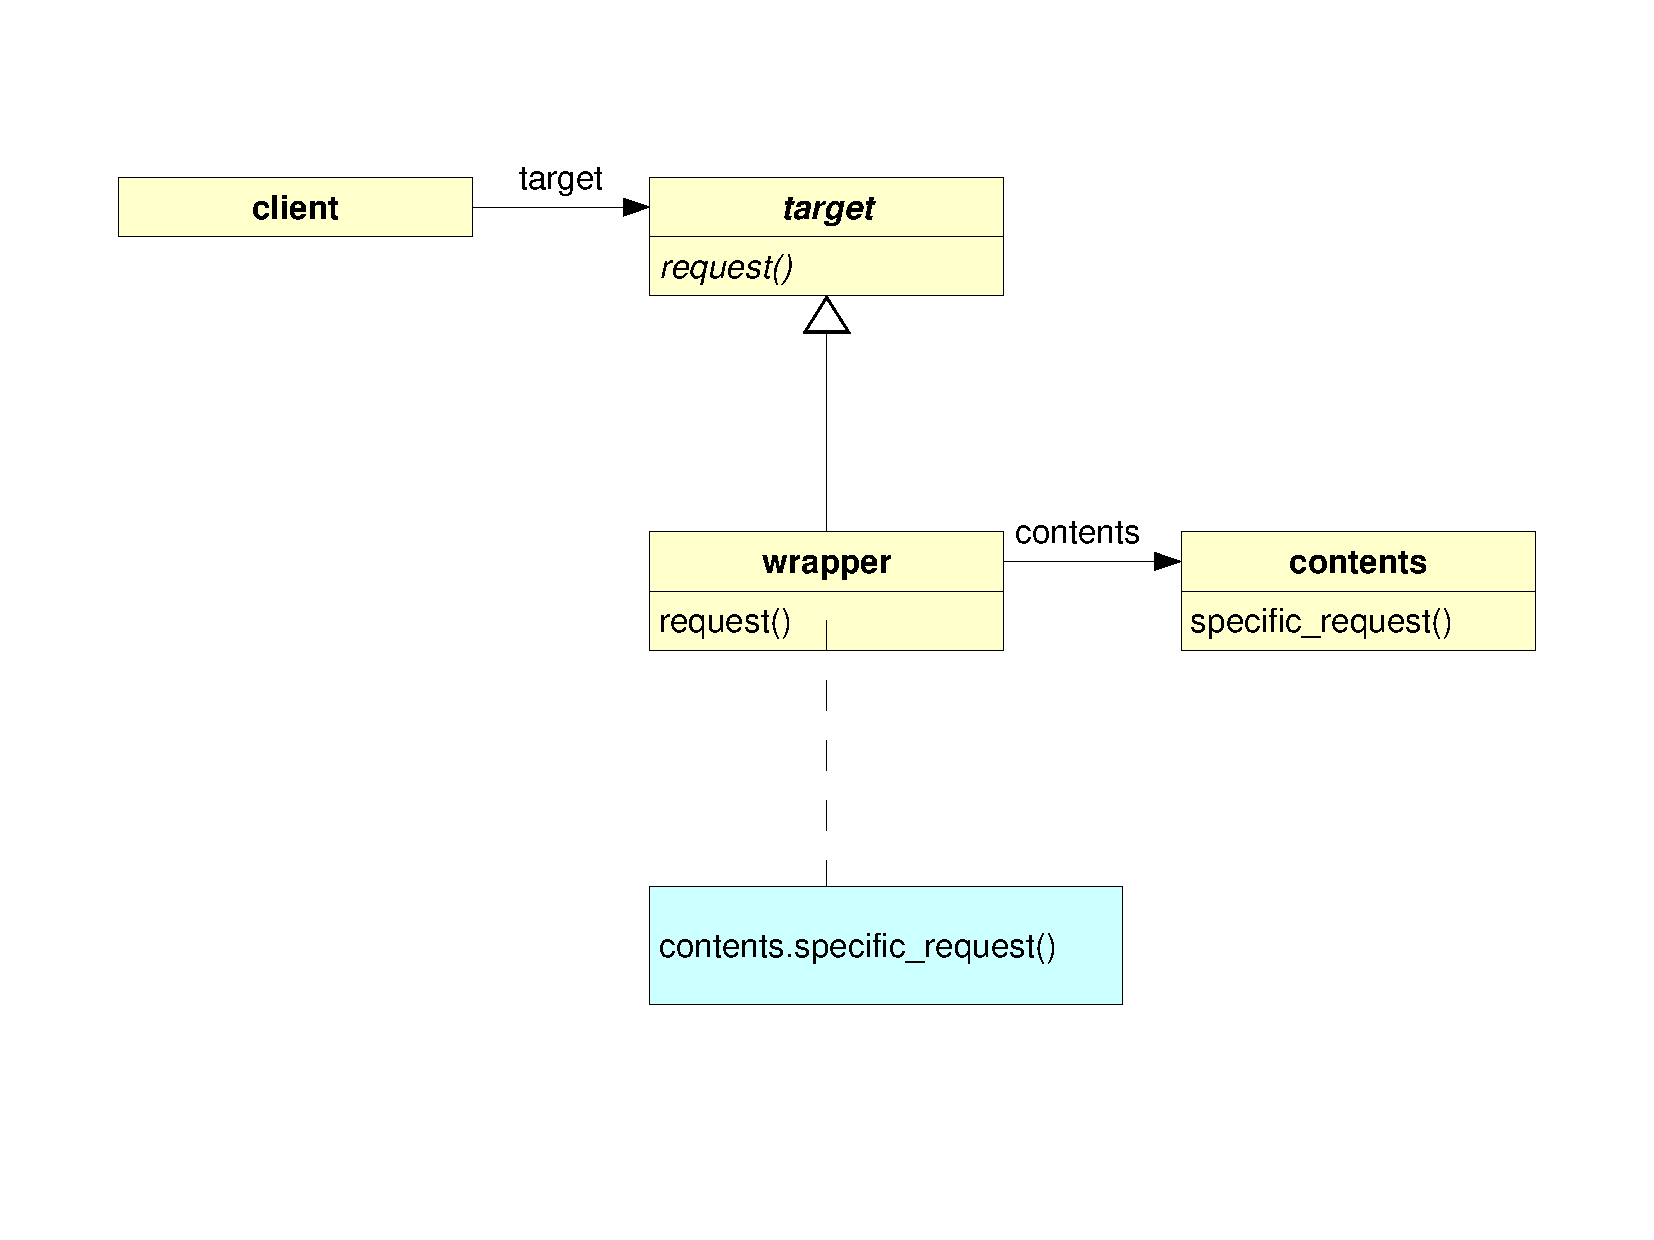
\includegraphics[scale=0.3,angle=-90]{graphic/wrapper.pdf}
        \caption{Wrapper Pattern}
        \label{wrapper_figure}
    \end{center}
\end{figure}

Knowledge templates created in the language described in chapter
\ref{cybernetics_oriented_language_heading} wrap the more fine-granular
templates they consist of.

%
% $RCSfile: whole_part.tex,v $
%
% Copyright (c) 2004. Christian Heller. All rights reserved.
%
% No copying, altering, distribution or any other actions concerning this
% document, except after explicit permission by the author!
% At some later point in time, this document is planned to be put under
% the GNU FDL license. For now, _everything_ is _restricted_ by the author.
%
% http://www.cybop.net
% - Cybernetics Oriented Programming -
%
% http://www.resmedicinae.org
% - Information in Medicine -
%
% @author Christian Heller <christian.heller@tuxtax.de>
%

\paragraph{Whole Part}
\label{whole_part_heading}

Whenever many components form a semantic unit, they can be subsumed by the
\emph{Whole-Part} pattern \cite{buschmann}. It encapsulates single part objects
(figure \ref{wholepart_figure}) and controls their cooperation. Part objects
are not addressable directly.

Almost all software systems contain components or sub systems which could be
organized by help of this pattern. In some way, it is quite similar to the
previously introduced \emph{Wrapper}, only that not just one- but many objects
are wrapped.

\begin{figure}[ht]
    \begin{center}
        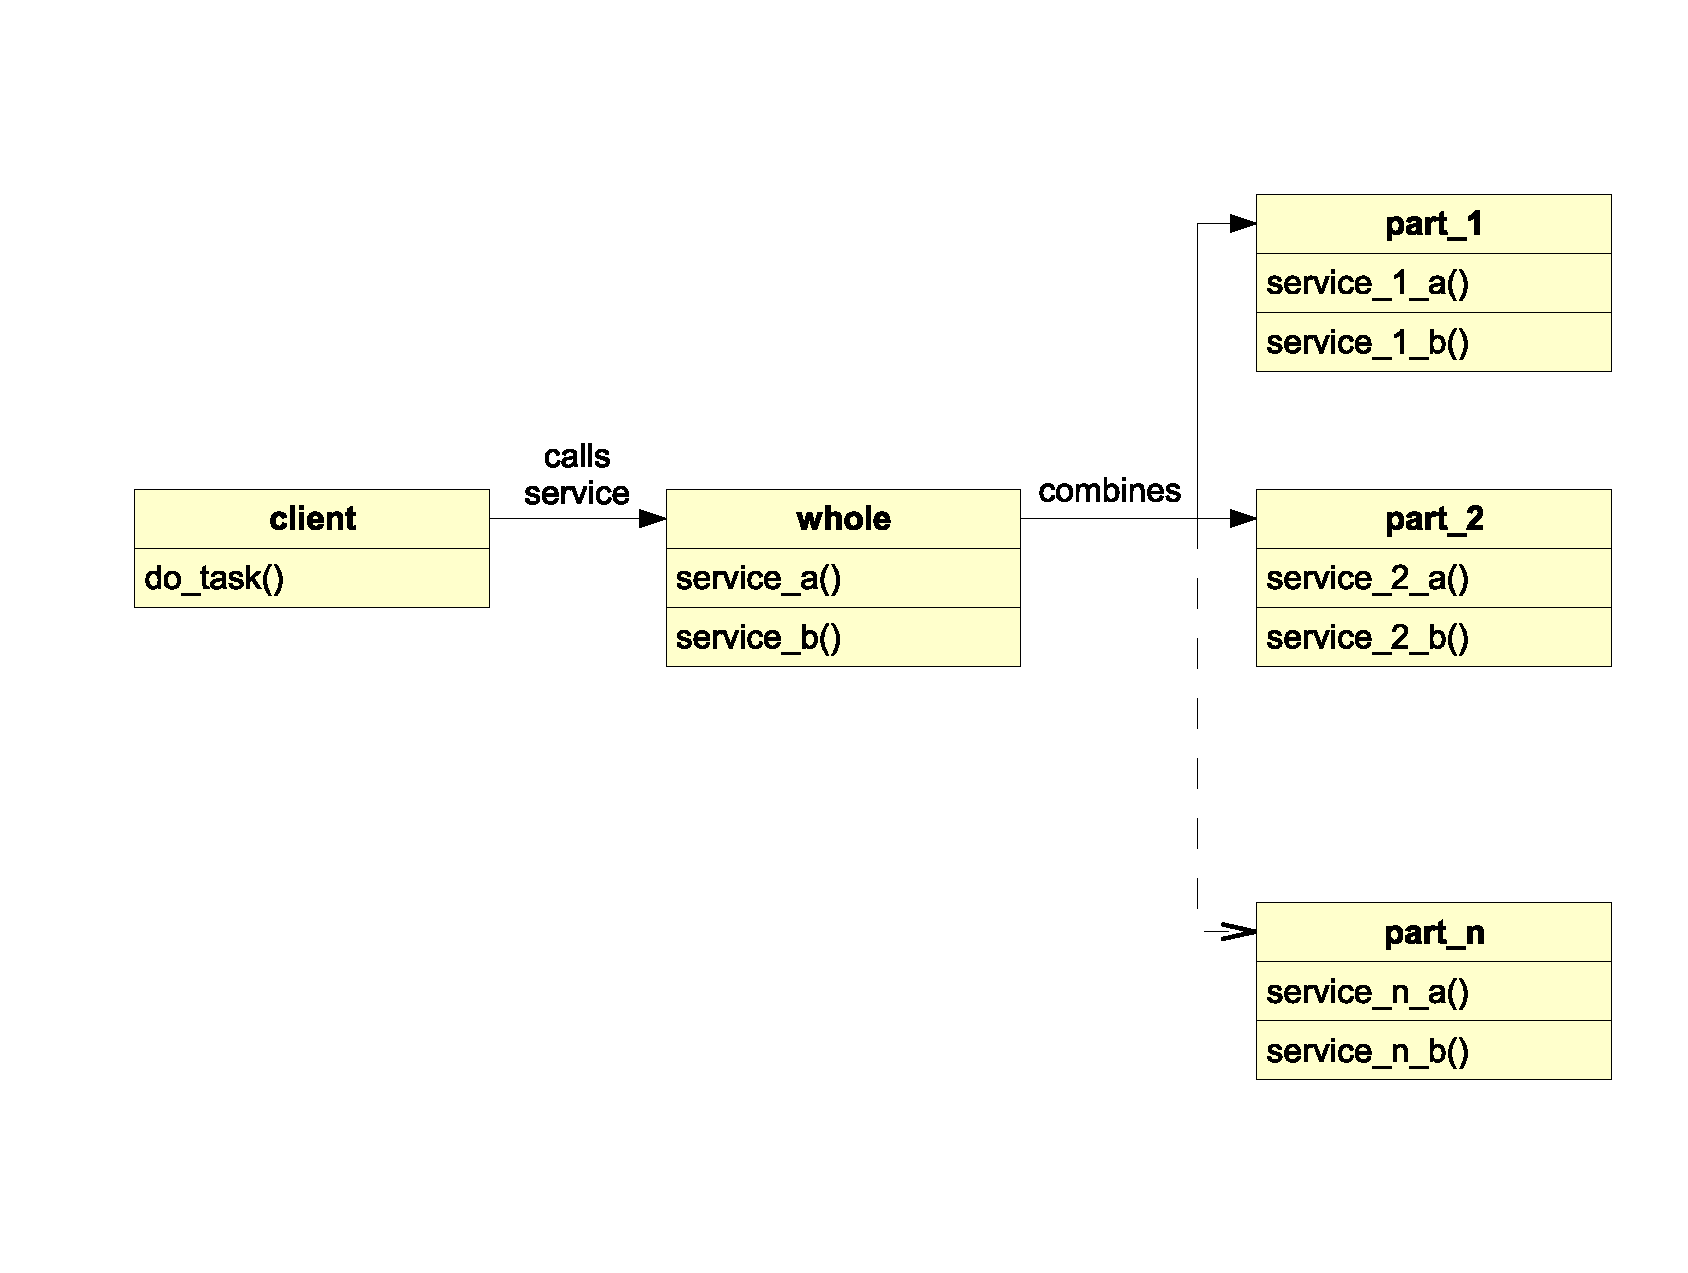
\includegraphics[scale=0.3]{vector/wholepart.eps}
        \caption{Whole-Part Pattern}
        \label{wholepart_figure}
    \end{center}
\end{figure}

%
% $RCSfile: composite.tex,v $
%
% Copyright (c) 2004. Christian Heller. All rights reserved.
%
% No copying, altering, distribution or any other actions concerning this
% document, except after explicit permission by the author!
% At some later point in time, this document is planned to be put under
% the GNU FDL license. For now, _everything_ is _restricted_ by the author.
%
% http://www.cybop.net
% - Cybernetics Oriented Programming -
%
% http://www.resmedicinae.org
% - Information in Medicine -
%
% @author Christian Heller <christian.heller@tuxtax.de>
%

\paragraph{Composite}
\label{composite_heading}

A hierarchical object structure, also called \emph{Directed Acyclical Graph}
(DAG) or \emph{Tree}, can be represented by a combination of classes called
\emph{Composite} pattern \cite{gamma1995}. It describes a \emph{Component} that
may consist of \emph{Children} (figure \ref{composite_figure}), which makes it
comparable to the \emph{Whole-Part} pattern. The difference is that the
\emph{Composite} is a more generalized version, with a dynamically extensible
number of child (part) objects.

The \emph{Composite} is a pattern based on \emph{Recursion}, which is one of
the most commonly used programming techniques at all. The pattern's split into
\emph{Leaf-} and \emph{Composite} sub classes helps distinguish primitive- from
container objects. A composite tree node holds objects of type \emph{Component}.

\begin{figure}[ht]
    \begin{center}
        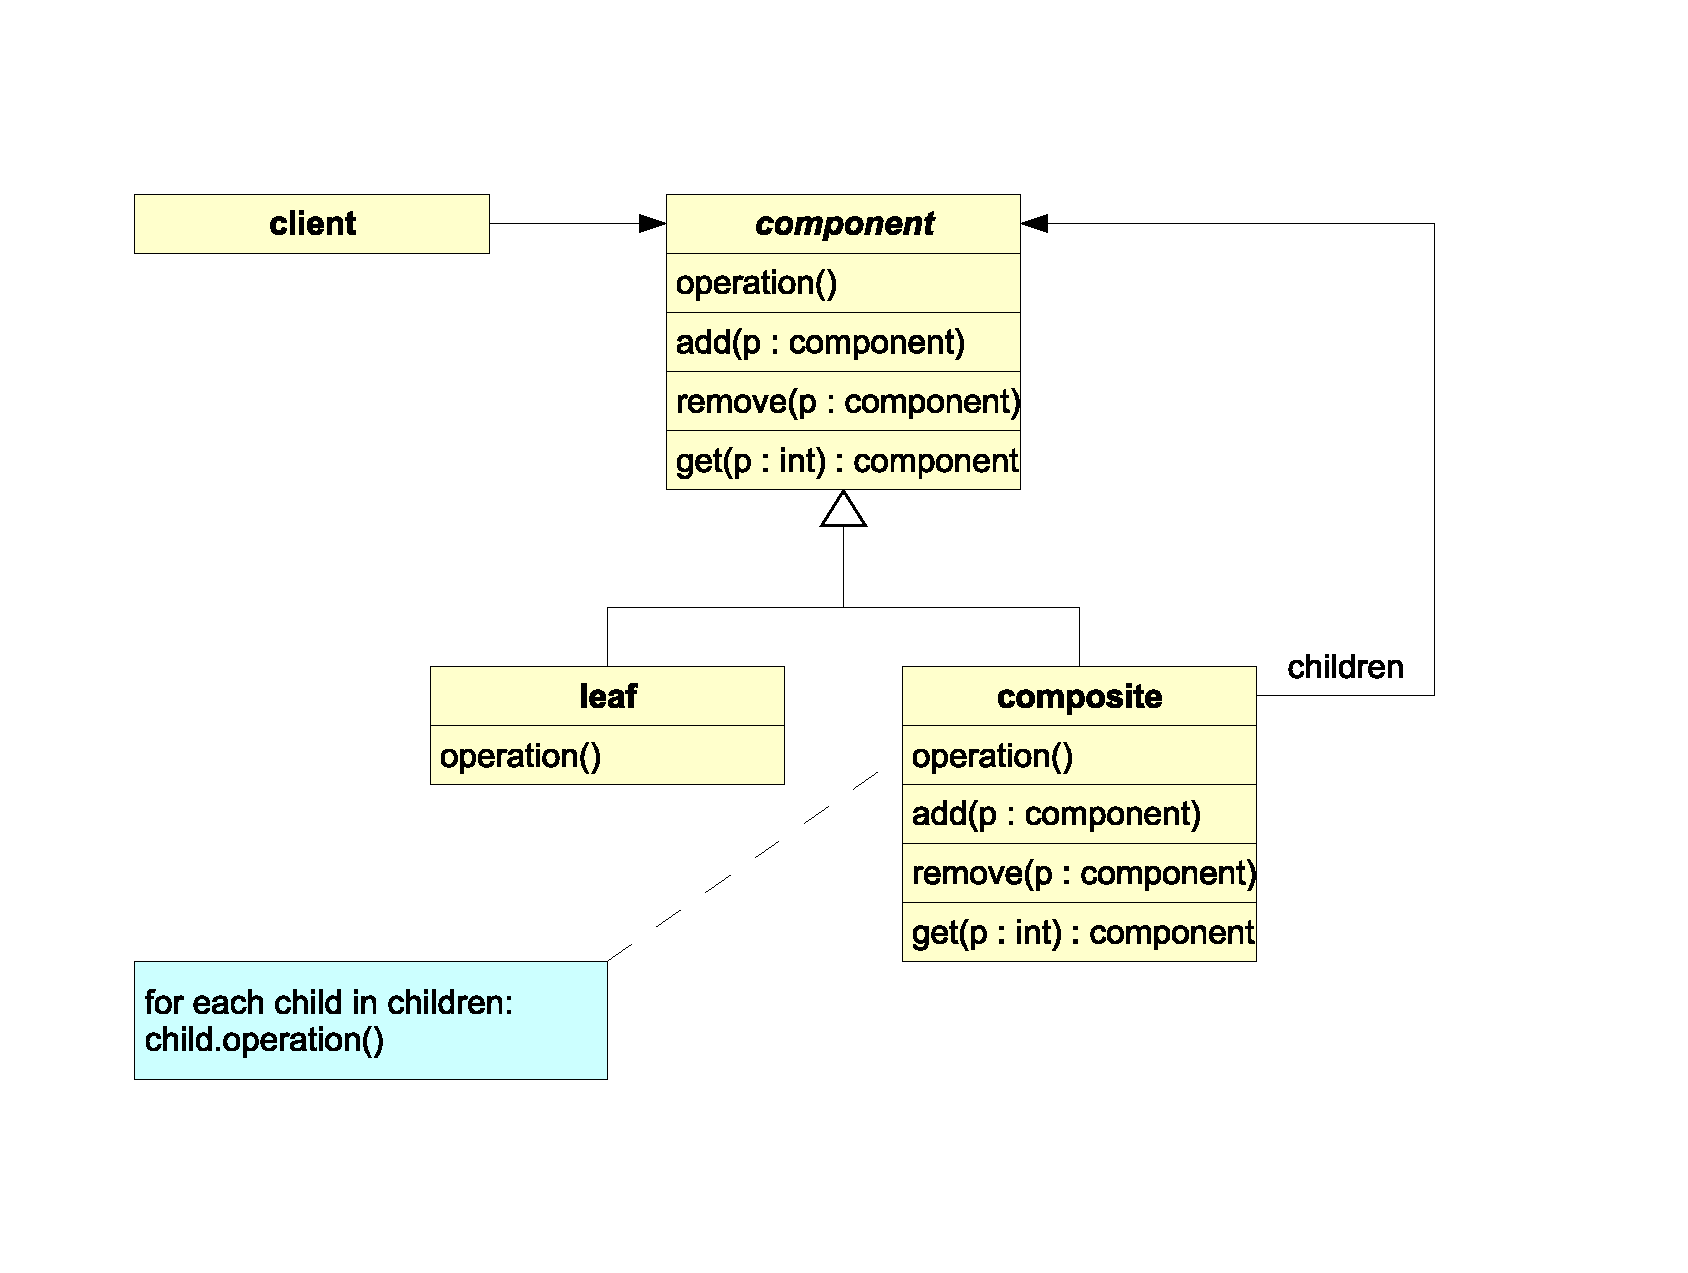
\includegraphics[scale=0.3]{vector/composite.eps}
        \caption{Composite Pattern}
        \label{composite_figure}
    \end{center}
\end{figure}

%
% $RCSfile: chain_of_responsibility.tex,v $
%
% Copyright (c) 2004. Christian Heller. All rights reserved.
%
% No copying, altering, distribution or any other actions concerning this
% document, except after explicit permission by the author!
% At some later point in time, this document is planned to be put under
% the GNU FDL license. For now, _everything_ is _restricted_ by the author.
%
% http://www.cybop.net
% - Cybernetics Oriented Programming -
%
% http://www.resmedicinae.org
% - Information in Medicine -
%
% @author Christian Heller <christian.heller@tuxtax.de>
%

\paragraph{Chain of Responsibility}
\label{chain_of_responsibility_heading}

The \emph{Chain of Responsibility} pattern \cite{gamma1995} is similar to the
\emph{Composite}, in that it represents a recursive structure as well. Objects
destined to solve a task are linked with a corresponding \emph{Successor}
(figure \ref{chain_figure}), such forming a chain. If an object is not able to
solve a task, that task is forwarded to the object's successor, along the chain.

\begin{figure}[ht]
    \begin{center}
        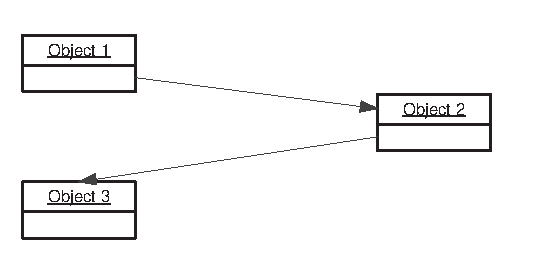
\includegraphics[scale=0.3]{vector/chain.eps}
        \caption{Chain of Responsibility Pattern}
        \label{chain_figure}
    \end{center}
\end{figure}

The pattern found wide application, for example in help systems, in event
handling frameworks or for exception handling. Its \emph{Handler} class is
known under synonyms like \emph{Event Handler}, \emph{Bureaucrat} or
\emph{Responder}.

Frequently, the pattern gets misused by delegating messages not only to children
but also to the parent of objects. The \emph{Hierarhical Model View Controller}
(HMVC) pattern is one example for this. It causes unfavourable bidirectional
dependencies (section \ref{bidirectional_dependency_heading}) and leads to
stronger coupling between the layers of a framework, because parent- and child
objects then reference each other.

%
% $RCSfile: observer.tex,v $
%
% Copyright (c) 2004. Christian Heller. All rights reserved.
%
% No copying, altering, distribution or any other actions concerning this
% document, except after explicit permission by the author!
% At some later point in time, this document is planned to be put under
% the GNU FDL license. For now, _everything_ is _restricted_ by the author.
%
% http://www.cybop.net
% - Cybernetics Oriented Programming -
%
% http://www.resmedicinae.org
% - Information in Medicine -
%
% @author Christian Heller <christian.heller@tuxtax.de>
%

\paragraph{Observer}
\label{observer_heading}

Another pattern that found wide application is the \emph{Observer} \cite{gamma1995},
an often-used synonym for which is \emph{Publisher-Subscriber}. It provides a
notification mechanism for all objects that registered as \emph{Observer} at a
\emph{Subject} in whose state changes they are interested, leading to an automatic
update of all dependent objects (figure \ref{observer_figure}).

\begin{figure}[ht]
    \begin{center}
        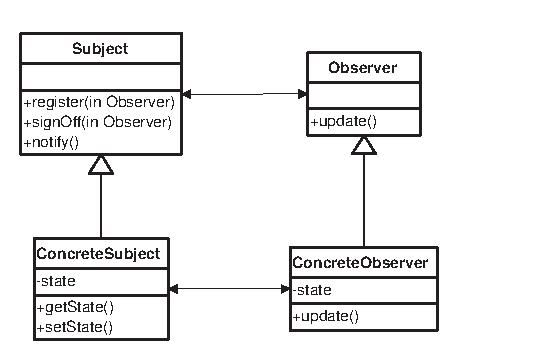
\includegraphics[scale=0.3]{vector/observer.eps}
        \caption{Observer Pattern}
        \label{observer_figure}
    \end{center}
\end{figure}

\begin{figure}[ht]
    \begin{center}
        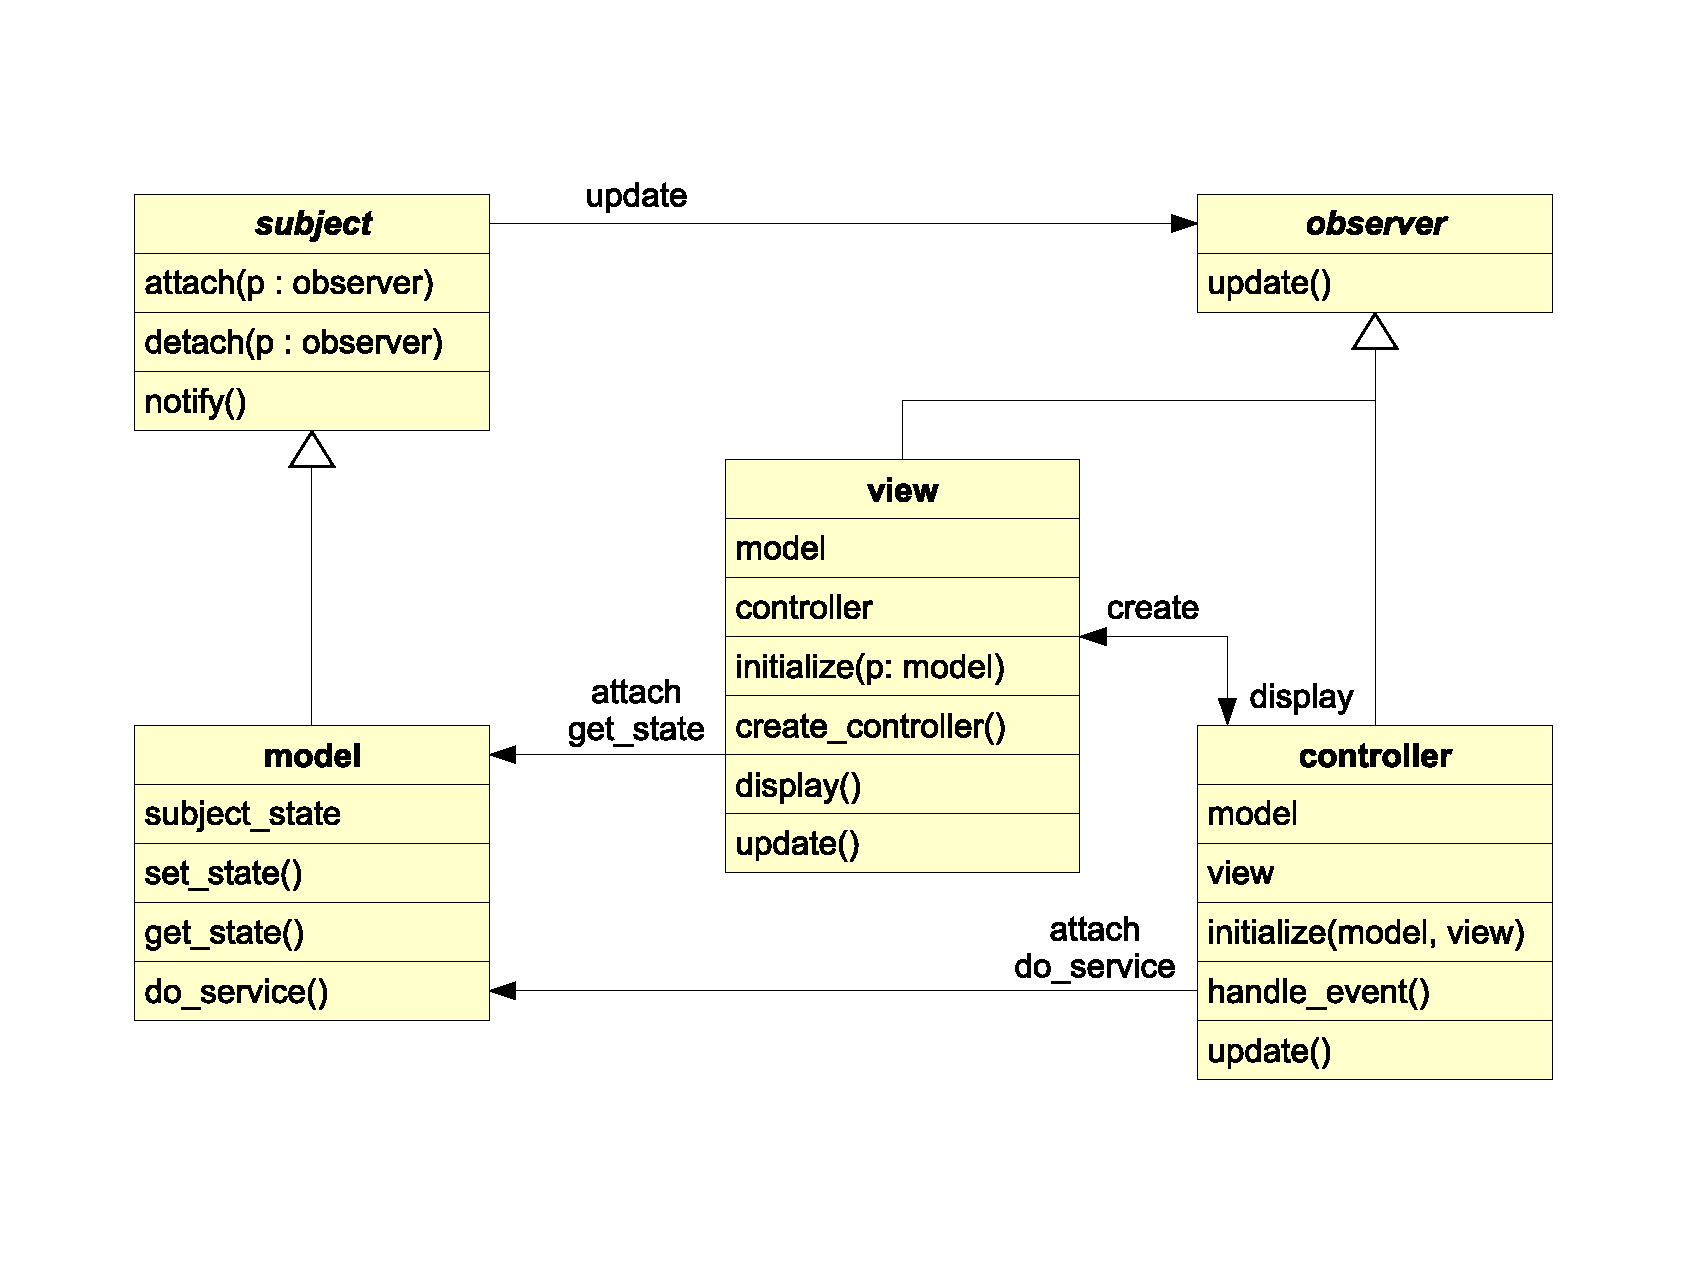
\includegraphics[scale=0.3]{vector/mvcobserver.eps}
        \caption{MVC- using Observer Pattern}
        \label{mvcobserver_figure}
    \end{center}
\end{figure}

Similar notification mechanisms are used for \emph{Callback} event handling in
frameworks, where the framework core calls functionality of its extensions. The
\emph{Model View Controller-} (MVC) uses the \emph{Observer} pattern to let the
model notify its observing views about necessary updates (figure
\ref{mvcobserver_figure}).

A disadvantage of the \emph{Observer} pattern is that it relies on bidirectional
dependencies (section \ref{bidirectional_dependency_heading}), so that circular
references can occur, when a system is not programmed very carefully.

%
% $RCSfile: bidirectional_dependency.tex,v $
%
% Copyright (C) 2002-2008. Christian Heller.
%
% Permission is granted to copy, distribute and/or modify this document
% under the terms of the GNU Free Documentation License, Version 1.1 or
% any later version published by the Free Software Foundation; with no
% Invariant Sections, with no Front-Cover Texts and with no Back-Cover
% Texts. A copy of the license is included in the section entitled
% "GNU Free Documentation License".
%
% http://www.cybop.net
% - Cybernetics Oriented Programming -
%
% http://www.resmedicinae.org
% - Information in Medicine -
%
% Version: $Revision: 1.1 $ $Date: 2008-08-19 20:41:05 $ $Author: christian $
% Authors: Christian Heller <christian.heller@tuxtax.de>
%

\subsubsection{Bidirectional Dependency}
\label{bidirectional_dependency_heading}
\index{Bidirectional Dependency}
\index{Inter-Dependency}
\index{Endless Loop}
\index{Tree}
\index{Directed Acyclic Graph}
\index{DAG}
\index{Oriented Acyclic Graph}
\index{Process Tree}
\index{Object Tree}
\index{Database Data Structure}
\index{File System Structure}
\index{Syntax Tree}
\index{Acyclic Graph}
\index{Circular Reference}

\emph{Bidirectional References} are a nightmare for every software developer.
They cause \emph{Inter-Dependencies} so that changes in one part of a system can
affect multiple other parts which in turn affect the originating part, which may
finally lead to cycles or even endless loops. Also, the actual program flow and
effects of changes to a system become very hard to trace. Therefore, the avoidance
of such dependencies belongs to the core principles of good software design.

A \emph{Tree}, in mathematics, is defined as \textit{Directed Acyclic Graph}
(DAG), also known as \emph{Oriented Acyclic Graph} \cite{nist}. It has a
\emph{Root Node} and \emph{Child Nodes} which can become \emph{Parent Nodes}
when having children themselves; otherwise they are called \emph{Leaves}.
Children of the same node are \emph{Siblings}. \textit{A common constraint is
that no node can have more than one parent}, as \cite{foldoc} writes and
continues: \textit{Moreover, for some applications, it is necessary to consider
a node's children to be an ordered list, instead of merely a set.} A graph is
\emph{acyclic} if every node can be reached via exactly one path, which then
also is the shortest possible.

In computing, trees are used in many forms, for example as \emph{Process Tree}
of an operating system \cite{debian, gnu, linux} or as \emph{Object Tree} of an
object-oriented application. They represent \emph{Data Structures} in databases
or file systems and also the \emph{Syntax Tree} of languages. The violation of
the principle of the \emph{Acyclic Graph} can lead to the same loops, also
called \emph{Circular References}, as mentioned above, which can result in the
crossing of memory limits and is a potential security risk. Therefore, one of
the main aims in the creation of the new concepts introduced in part
\ref{contribution_heading} of this work was the avoidance of bidirectional
relations.


%
% $RCSfile: idiomatic.tex,v $
%
% Copyright (C) 2002-2008. Christian Heller.
%
% Permission is granted to copy, distribute and/or modify this document
% under the terms of the GNU Free Documentation License, Version 1.1 or
% any later version published by the Free Software Foundation; with no
% Invariant Sections, with no Front-Cover Texts and with no Back-Cover
% Texts. A copy of the license is included in the section entitled
% "GNU Free Documentation License".
%
% http://www.cybop.net
% - Cybernetics Oriented Programming -
%
% http://www.resmedicinae.org
% - Information in Medicine -
%
% Version: $Revision: 1.1 $ $Date: 2008-08-19 20:41:07 $ $Author: christian $
% Authors: Christian Heller <christian.heller@tuxtax.de>
%

\subsection{Idiomatic}
\label{idiomatic_heading}
\index{Idiomatic Pattern}
\index{Idiom}
\index{Counted Pointer Pattern}
\index{Singleton Pattern}
\index{Template Method Pattern}
\index{Factory Method Pattern}
\index{Envelope Letter Pattern}

An \emph{Idiom} is a pattern on a low abstraction level. It describes how certain
aspects of components or the relations between them can be implemented using the
means of a specific programming language. Idioms can thus be used to describe
the actual realisation of design patterns. Besides the \emph{Counted-Pointer}
pattern, Buschmann \cite[p. 377]{buschmann} also categorises \emph{Singleton},
\emph{Template Method}, \emph{Factory Method} and \emph{Envelope-Letter}
\cite{coplien} as \emph{Idiom}.

%
% $RCSfile: template_method.tex,v $
%
% Copyright (C) 2002-2008. Christian Heller.
%
% Permission is granted to copy, distribute and/or modify this document
% under the terms of the GNU Free Documentation License, Version 1.1 or
% any later version published by the Free Software Foundation; with no
% Invariant Sections, with no Front-Cover Texts and with no Back-Cover
% Texts. A copy of the license is included in the section entitled
% "GNU Free Documentation License".
%
% http://www.cybop.net
% - Cybernetics Oriented Programming -
%
% http://www.resmedicinae.org
% - Information in Medicine -
%
% Version: $Revision: 1.1 $ $Date: 2008-08-19 20:41:09 $ $Author: christian $
% Authors: Christian Heller <christian.heller@tuxtax.de>
%

\subsubsection{Template Method}
\label{template_method_heading}
\index{Template Method Pattern}
\index{Hook Method Pattern}

The \emph{Template Method} pattern \cite{gamma1995}, also called
\emph{Hook Method}, is an abstract definition of the \emph{Skeleton} of an
algorithm. The implementation of one or more steps of that algorithm is
delegated to a sub class (figure \ref{templatemethod_figure}).

\begin{figure}[ht]
    \begin{center}
        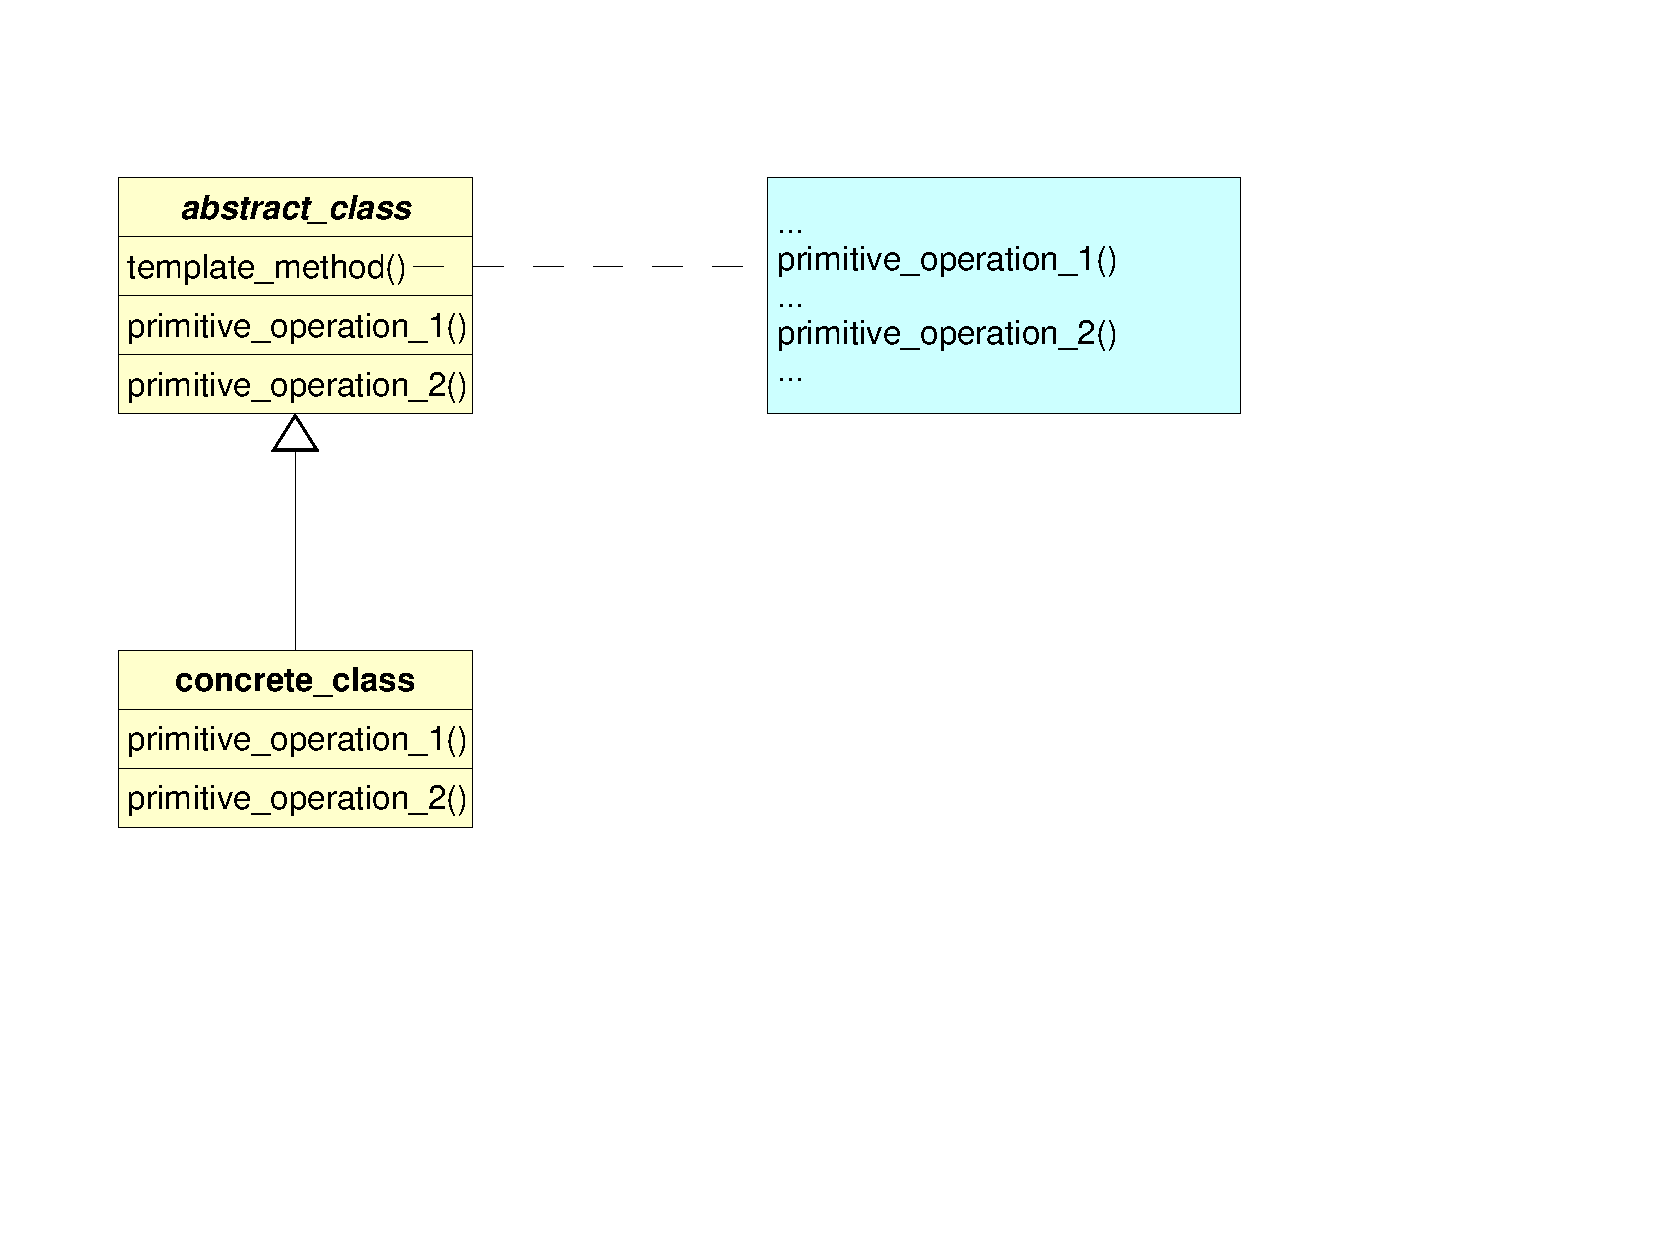
\includegraphics[scale=0.3,angle=-90]{graphic/templatemethod.pdf}
        \caption{Template Method Pattern}
        \label{templatemethod_figure}
    \end{center}
\end{figure}

The idea of algorithm (method) templates was taken over in the design of the
new language described in chapter \ref{cybernetics_oriented_language_heading}.
The single template parts, however, are not inherited but implemented in
\emph{part} templates referenced by their corresponding \emph{whole} template,
which is actually more similar to the previously described \emph{Whole-Part}
pattern (section \ref{design_heading}).

%
% $RCSfile: counted_pointer.tex,v $
%
% Copyright (c) 2004. Christian Heller. All rights reserved.
%
% No copying, altering, distribution or any other actions concerning this
% document, except after explicit permission by the author!
% At some later point in time, this document is planned to be put under
% the GNU FDL license. For now, _everything_ is _restricted_ by the author.
%
% http://www.cybop.net
% - Cybernetics Oriented Programming -
%
% http://www.resmedicinae.org
% - Information in Medicine -
%
% @author Christian Heller <christian.heller@tuxtax.de>
%

\paragraph{Counted Pointer}
\label{counted_pointer_heading}

The \emph{Counted Pointer} pattern \cite{buschmann} supports memory management
in the \emph{C++} programming language, by counting references to dynamically
created objects (figure \ref{pointer_figure}). That way, it can avoid the
destruction of an object through one client, while still being referenced by
other clients. Also, it helps avoiding memory leaks by cleaning up forgotten
objects.

\begin{figure}[ht]
    \begin{center}
        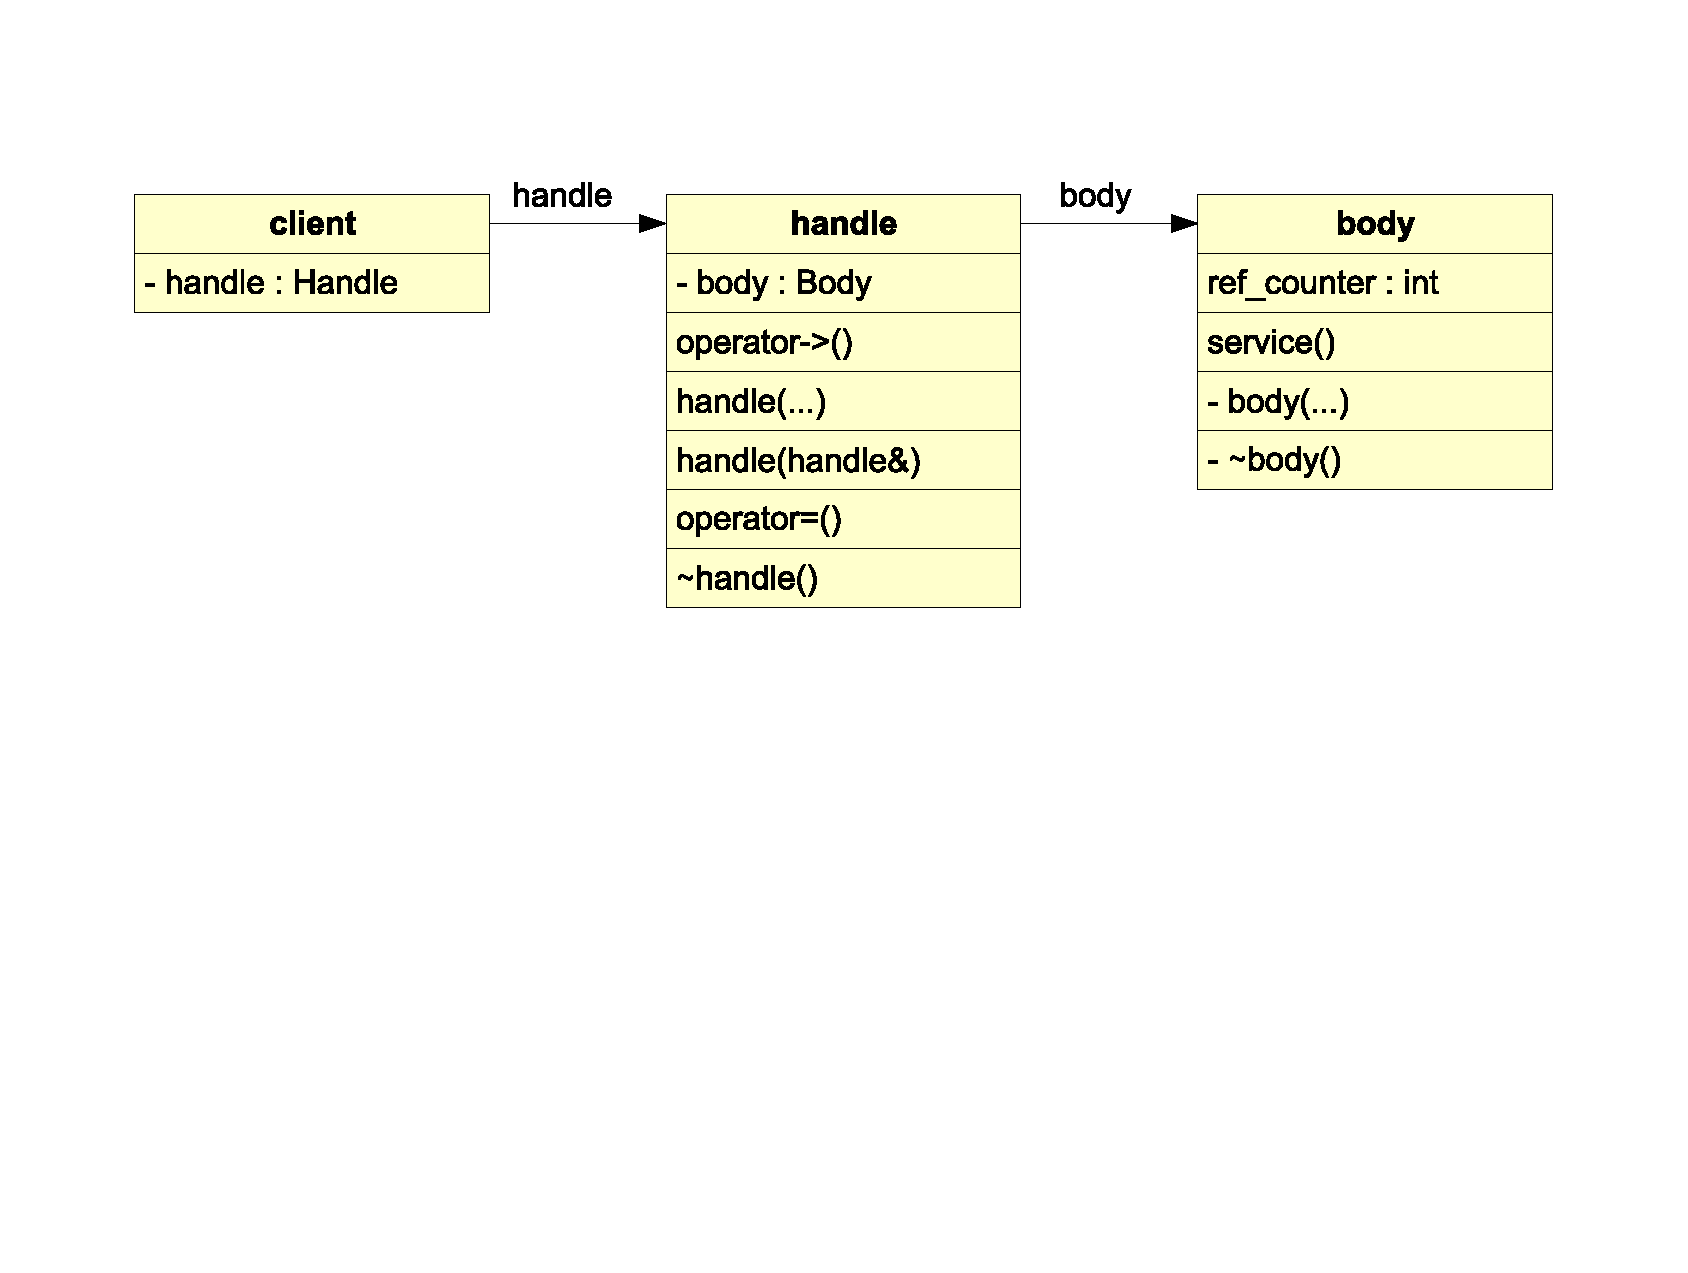
\includegraphics[scale=0.3]{vector/pointer.eps}
        \caption{Counted Pointer Pattern}
        \label{pointer_figure}
    \end{center}
\end{figure}

%
% $RCSfile: singleton.tex,v $
%
% Copyright (C) 2002-2008. Christian Heller.
%
% Permission is granted to copy, distribute and/or modify this document
% under the terms of the GNU Free Documentation License, Version 1.1 or
% any later version published by the Free Software Foundation; with no
% Invariant Sections, with no Front-Cover Texts and with no Back-Cover
% Texts. A copy of the license is included in the section entitled
% "GNU Free Documentation License".
%
% http://www.cybop.net
% - Cybernetics Oriented Programming -
%
% http://www.resmedicinae.org
% - Information in Medicine -
%
% Version: $Revision: 1.1 $ $Date: 2008-08-19 20:41:08 $ $Author: christian $
% Authors: Christian Heller <christian.heller@tuxtax.de>
%

\subsubsection{Singleton}
\label{singleton_heading}
\index{Singleton Pattern}
\index{Global Data Access}
\index{Class Method}
\index{Registry Object Pattern}
\index{Manager Object Pattern}
\index{Lifecycle Method}

Whenever an object-oriented system wants to ensure that only one instance of a
certain class exists, the \emph{Singleton} pattern \cite{gamma1995} can be
used. It essentially is a class which encapsulates its instance's data and
provides global access to them, via \emph{static}, sometimes called
\emph{class} methods (figure \ref{singleton_figure}).

\begin{figure}[ht]
    \begin{center}
        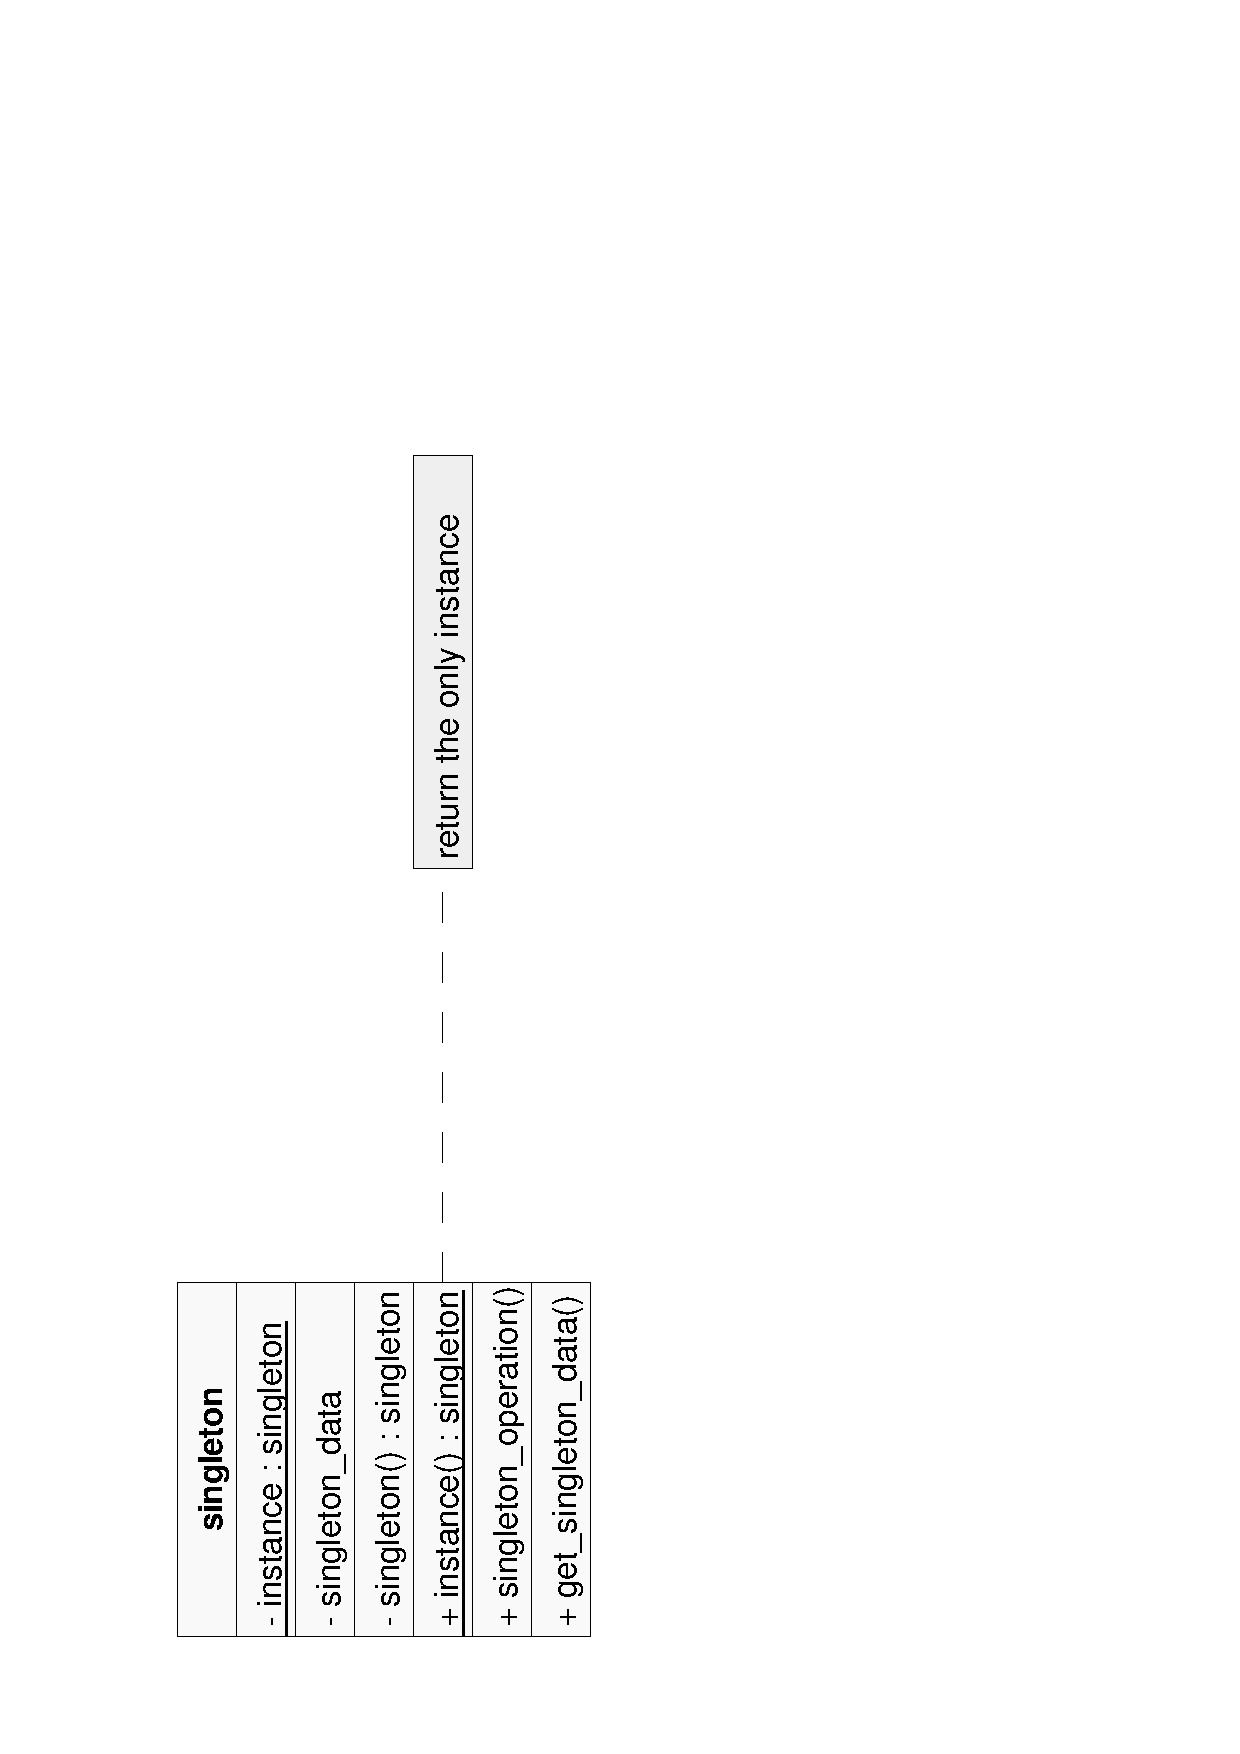
\includegraphics[scale=0.3,angle=-90]{graphic/singleton.pdf}
        \caption{Singleton Pattern}
        \label{singleton_figure}
    \end{center}
\end{figure}

A \emph{Registry} object as described by Fowler \cite{fowler2002} often uses
the \emph{Singleton} pattern, to be unique and to become globally accessible.
Similarly do many so-called \emph{Manager} objects, for example change managers
which are also responsible for the caching of objects.

Global, that is static access -- the main purpose of the \emph{Singleton}
pattern, is its main weakness, at the same time. One obvious solution to avoid
singleton objects could be to forward global information as instances from
component to component, possibly using an own \emph{Lifecycle Method} (section
\ref{component_lifecycle_heading}). This approach, however, might bring with a
rather large number of parameters to be handed over. It therefore seems easier
to use another alternative -- the central tree of knowledge instances, as done
in the interpreter of chapter \ref{cybernetics_oriented_interpreter_heading}.

%
% $RCSfile: global_access.tex,v $
%
% Copyright (c) 2004. Christian Heller. All rights reserved.
%
% No copying, altering, distribution or any other actions concerning this
% document, except after explicit permission by the author!
% At some later point in time, this document is planned to be put under
% the GNU FDL license. For now, _everything_ is _restricted_ by the author.
%
% http://www.cybop.net
% - Cybernetics Oriented Programming -
%
% http://www.resmedicinae.org
% - Information in Medicine -
%
% @author Christian Heller <christian.heller@tuxtax.de>
%

\subsection{Global Access}
\label{global_access_heading}

A pure tree of instances in a computer's \emph{Random Access Memory} (RAM)
represents an unidirectional structure that permits data access along
\emph{well-defined} paths. Global access via static types, on the other hand,
allows \emph{any} instance to address data in memory \emph{directly}, which not
only complicates software development and maintenance, but, due to the
uncontrollable access, is a potential security risk.

The usage of static objects accessible by any other part in a system is an
\emph{Anti Pattern} to \emph{Inversion of Control} (IoC) \cite{avalon}, highly
insecure and hence undesirable.


%
% $RCSfile: framework.tex,v $
%
% Copyright (C) 2002-2008. Christian Heller.
%
% Permission is granted to copy, distribute and/or modify this document
% under the terms of the GNU Free Documentation License, Version 1.1 or
% any later version published by the Free Software Foundation; with no
% Invariant Sections, with no Front-Cover Texts and with no Back-Cover
% Texts. A copy of the license is included in the section entitled
% "GNU Free Documentation License".
%
% http://www.cybop.net
% - Cybernetics Oriented Programming -
%
% http://www.resmedicinae.org
% - Information in Medicine -
%
% Version: $Revision: 1.1 $ $Date: 2008-08-19 20:41:06 $ $Author: christian $
% Authors: Christian Heller <christian.heller@tuxtax.de>
%

\subsection{Framework}
\label{framework_heading}
\index{Framework}
\index{Software Framework}
\index{Pattern}
\index{Base Architecture}
\index{Library}
\index{Callback Mechanism}
\index{Inheritance}
\index{Polymorphism}
\index{Static Constraints of a Framework}
\index{Dynamic Parts of a Framework}
\index{Frozen Spot}
\index{Hot Spot}
\index{Contract}
\index{Vertical Market Framework}
\index{Horizontal Market Framework}
\index{Java Development Kit}
\index{JDK}
\index{Collection Framework}
\index{Input Method Framework}
\index{Bidirectional Dependency}
\index{Observer Pattern}
\index{Manager Class}
\index{Singleton Pattern}

In the past decade, \emph{Software Frameworks} have gained in importance.
Patterns are considered their elementary building blocks. Yet while patterns
are solutions for recurring design problems, frameworks represent the base
architecture for a family of systems \cite{pree}. Because both concepts depend
on each other, frameworks are described within the main section \emph{Patterns}.

A \emph{Framework} essentially is a reusable collection of a number of
cooperating abstract and concrete classes, in a special constellation. It
represents an imcomplete software system which still needs to be extended and
instantiated, to be executable. A conventional \emph{Library} is used by
calling the procedures provided by it; the main part of each application is
then designed and realised by the developer. A \emph{Framework} already
represents the actual main part of a system. Functionality added by the
application developer is reversely called and used by the framework itself.
This principle carries the name \emph{Callback Mechanism}. Extensions are
mostly realised through \emph{Inheritance} and \emph{Polymorphism} (section
\ref{object_oriented_programming_heading}).

But not all parts of a framework are intended to be extended. After W. Pree
\cite{pree}, there are \emph{Static Constraints} and \emph{Dynamic Parts}.
Buschmann \cite{buschmann} calls them \emph{Frozen Spots} and \emph{Hot Spots};
the \emph{Apache Jakarta Avalon} framework \cite{avalon} labels static parts
\emph{Contracts}. When the abstract state of a framework is turned into a
functioning application by instantiating its classes, static elements remain
unchanged. They form the basic structure for all derived applications.
Application-specific behaviour, on the other hand, is determined by
specialising adaptable framework parts.

The \emph{Jakarta Avalon} documentation \cite{avalon} defines a framework as:

\begin{enumerate}
    \item A supporting or enclosing structure.
    \item A basic system or arrangement as of ideas.
\end{enumerate}

It distinguishes between \emph{Vertical Market Frameworks} which focused on a
single industry like medical systems or telecommunications and would not work
well in other industries, and \emph{Horizontal Market Frameworks} which were
generic enough to be used across multiple industries. Vertical market frameworks
could be built on top of horizontal market frameworks.

Just like patterns, frameworks provide higher flexibility to software components,
prevent code duplication and lower development efforts \cite{pree}. Developers
are freed from frequently reinventing the same solutions and can concentrate on
actual application development. The similar structure of applications that base
on the same framework ensures consistency and eases their maintenance, and also
reduces the time it takes for a developer to learn how the software works. Of
course, the necessary adjustment for new developers should not be underestimated;
comprehensive documentation is necessary. But once the principles behind a
framework are understood, one will be able to comprehend any system built upon it.

The \emph{Java Development Kit} (JDK) \cite{java}, for example, offers a number of
special \emph{Collection} containers (section \ref{container_heading}) which it
calls \emph{Collection Framework}; there is also an \emph{Input Method Framework}
and so on. Over the years, however, the framework definition has become a bit
fuzzy here-and-there.

The price of framework reusability is \emph{Lower Flexibility}, which is due to
the above-mentioned static parts. Besides this, applications are subject to the
evolution of the underlying framework. However, that disadvantage shouldn't be
too bold, if the framework is designed general and clever enough.

Framework callback mechanisms rely on \emph{Bidirectional Dependencies} and bring
with all their disadvantages (section \ref{bidirectional_dependency_heading}). To
explain this briefly: Instances that want to be called by the framework need to
register at a caller before, as was explained in section \ref{observer_heading},
on the example of the \emph{Observer} pattern. In order to be able to register
themselves, callees need to know about the caller. Once callees are registered,
the caller knows about them in turn.

Frequently, statically accessible classes, also called \emph{Managers}, have to
be introduced to a framework, mostly due to unforeseen requirements. They often
use the \emph{Singleton} pattern (section \ref{singleton_heading}) to become
unique within a system. Managers of that kind serve as gateway to certain areas
of the framework that are not easily reachable anymore through normal navigation
along object associations. A number of negative effects related to static object
access were already mentioned (section \ref{global_access_heading}).

Chapter \ref{knowledge_schema_heading} introduces a structure called
\emph{Knowledge Schema} which, although being static, is capable of
representing general knowledge, thus allowing the creation of flexible
application systems. Bidirectional dependencies and global model (object)
access are not an issue in the new language and interpreter introduced in
chapters \ref{cybernetics_oriented_language_heading} and
\ref{cybernetics_oriented_interpreter_heading}, because any runtime knowledge
model may be accessed along well-defined paths in a simple tree-like structure.

